% !TEX root = thesis.tex

{
\cleardoublepage% Move to first page of new chapter
\let\cleardoublepage\relax% Don't allow page break
\noindent \small{Based on: \emph{A tale of two tails: insights from simulations into the formation of the peculiar dwarf galaxy NGC~1427A}, Mastropietro~M., De Rijcke~S., Peletier~R.F. \citet{Mastropietro2021}
}
\chapter[A tale of two tails: on the formation of NGC~1427A]{Insights from simulations into the formation of the peculiar dwarf galaxy NGC~1427A}
\label{ch:ngc1427a}
}

\abstract{
We present a scenario for the formation and the morphology of the arrow-shaped dwarf irregular galaxy NGC~1427A in the Fornax Cluster.
This galaxy shows intriguing stellar and gaseous tails pointing in different directions for which alternative but not conclusive formation scenarios have been proposed in the literature.
We performed $N$-body/SPH simulations of dwarf galaxies falling into a model of the Fornax cluster, exhibiting a jellyfish-like appearance while undergoing ram-pressure stripping.
We noted that some of our models show interesting tail morphologies similar to that of NGC~1427A.
In this way, the peculiar NGC~1427A structure can be studied using models whose stellar and neutral gas photometry and kinematics are in good agreement with the observed ones, without the need of invoking an interaction with a nearby galaxy.
Thanks to the tails, we can identify the requirements for a galaxy to expose such a structure and assess the possible position and velocity of the galaxy in the cluster.
This puts constraints on the orbit of the galaxy, its position in the cluster and the time since its pericenter passage.
From the statistics of identified snapshots following our modelling, we found that the most likely position of the galaxy is around $200$~kpc in front of the cluster center,
travelling towards the cluster with a velocity angle with respect to the line-of-sight direction of around $50$~deg.
This analysis can be useful in future observations of similar galaxies in clusters to characterise their position and velocity in the cluster and their formation.
}


\begin{figure*}
\centering
\includegraphics[width=\textwidth]{NGC1427A-crop.png}
\caption{False-colour image of NGC 1427A, based on HST Advanced Camera for Surveys (ACS) archival data (Proposal ID: 9689; PI: M. Gregg).
The following colour bands were used: blue=475W; green=775W; red=625W+660N (stellar emission was subtracted from the 660N image using a scaled 775W image).
This colour scheme makes the H$\alpha$ emission stand out in red. An asinh stretch was applied to bring out also the faint details.
The inset zooms in on the Northern Clump, showing it to be composed of two loose stellar clusters with embedded \Hii{} emission.
The Northern Clump also appears to be connected to the north-west rim of NGC 1427A's main body via a tenuous stream of stars.
The directions of the \Hi{} tail and towards the Fornax Cluster center are indicated with arrows.
The dotted ellipse is the same as in Figures 1 and 2 of \citet{Lee-Waddell2018} and indicates the shape and direction of the faint outskirts of the galaxy, which are quite distinct from the system's inner, brighter parts.
}
\label{fig:NGC1427A}
\end{figure*}
The distorted optical appearance and gaseous tails and overall jellyfish-like morphology --~barring currently active star formation in the gas tails~-- of NGC~1427A (Figure~\ref{fig:NGC1427A}) seems to be straightforwardly and satisfactorily explained by ram-pressure stripping in conjunction with cluster tidal forces.
In particular, as has been explored more in detail in Chapter \ref{ch:sim_results}, star formation flickers on and off inside the gaseous tails of simulated ram-pressure stripped dwarf galaxies as gas clumps condense and disperse again.
This gives the label ``jellyfish galaxy" a transient and possibly recurrent quality.

To correctly interpret the available data, it is of prime importance to be able to reliably identify the dominant transformation process for this galaxy.
With this goal in mind, we compare recent \Hi{} and optical data of NGC~1427A with a suite of dwarf galaxy simulations, set in a Fornax Cluster environment.

In the next section, we give a short overview of the observed properties of NGC~1427A and focus on those that are considered most relevant for elucidating its origin and evolution.
The methodology behind the comparison of these simulations with the observations is discussed in Section~\ref{sec:results}.
We conclude with a discussion of the main results in Section~\ref{sec:discussion}.


\section{Observed properties of NGC~1427A} \label{sec:observations}
\begin{figure*}
\centering
\begin{subfigure}[b]{0.49\textwidth}
  \centering
  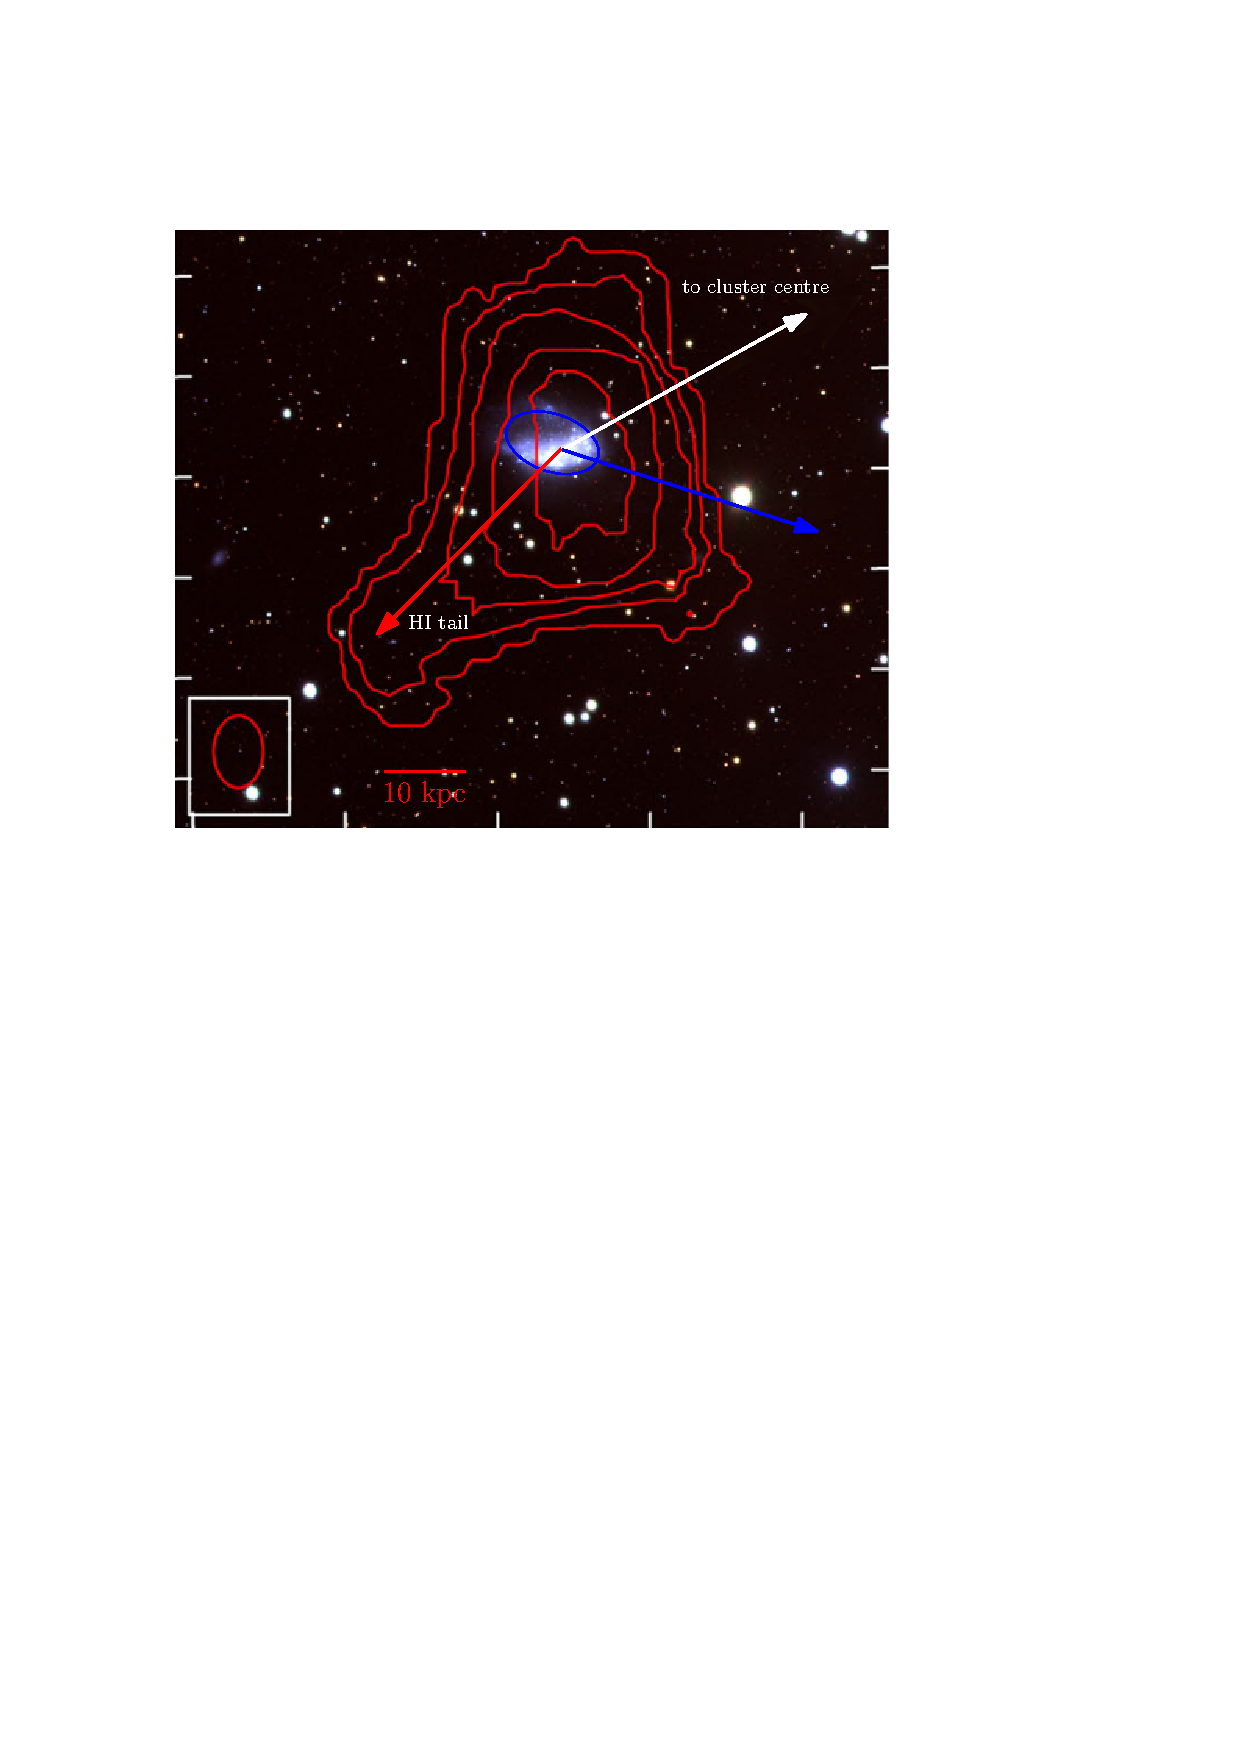
\includegraphics[width=\textwidth]{NGC_LIKE/ngc_location_scale.pdf}\\[3ex]
  \caption{}
  \label{fig:hi_contours}
\end{subfigure}
% \hfill
\begin{subfigure}[b]{0.49\textwidth}
  \centering
  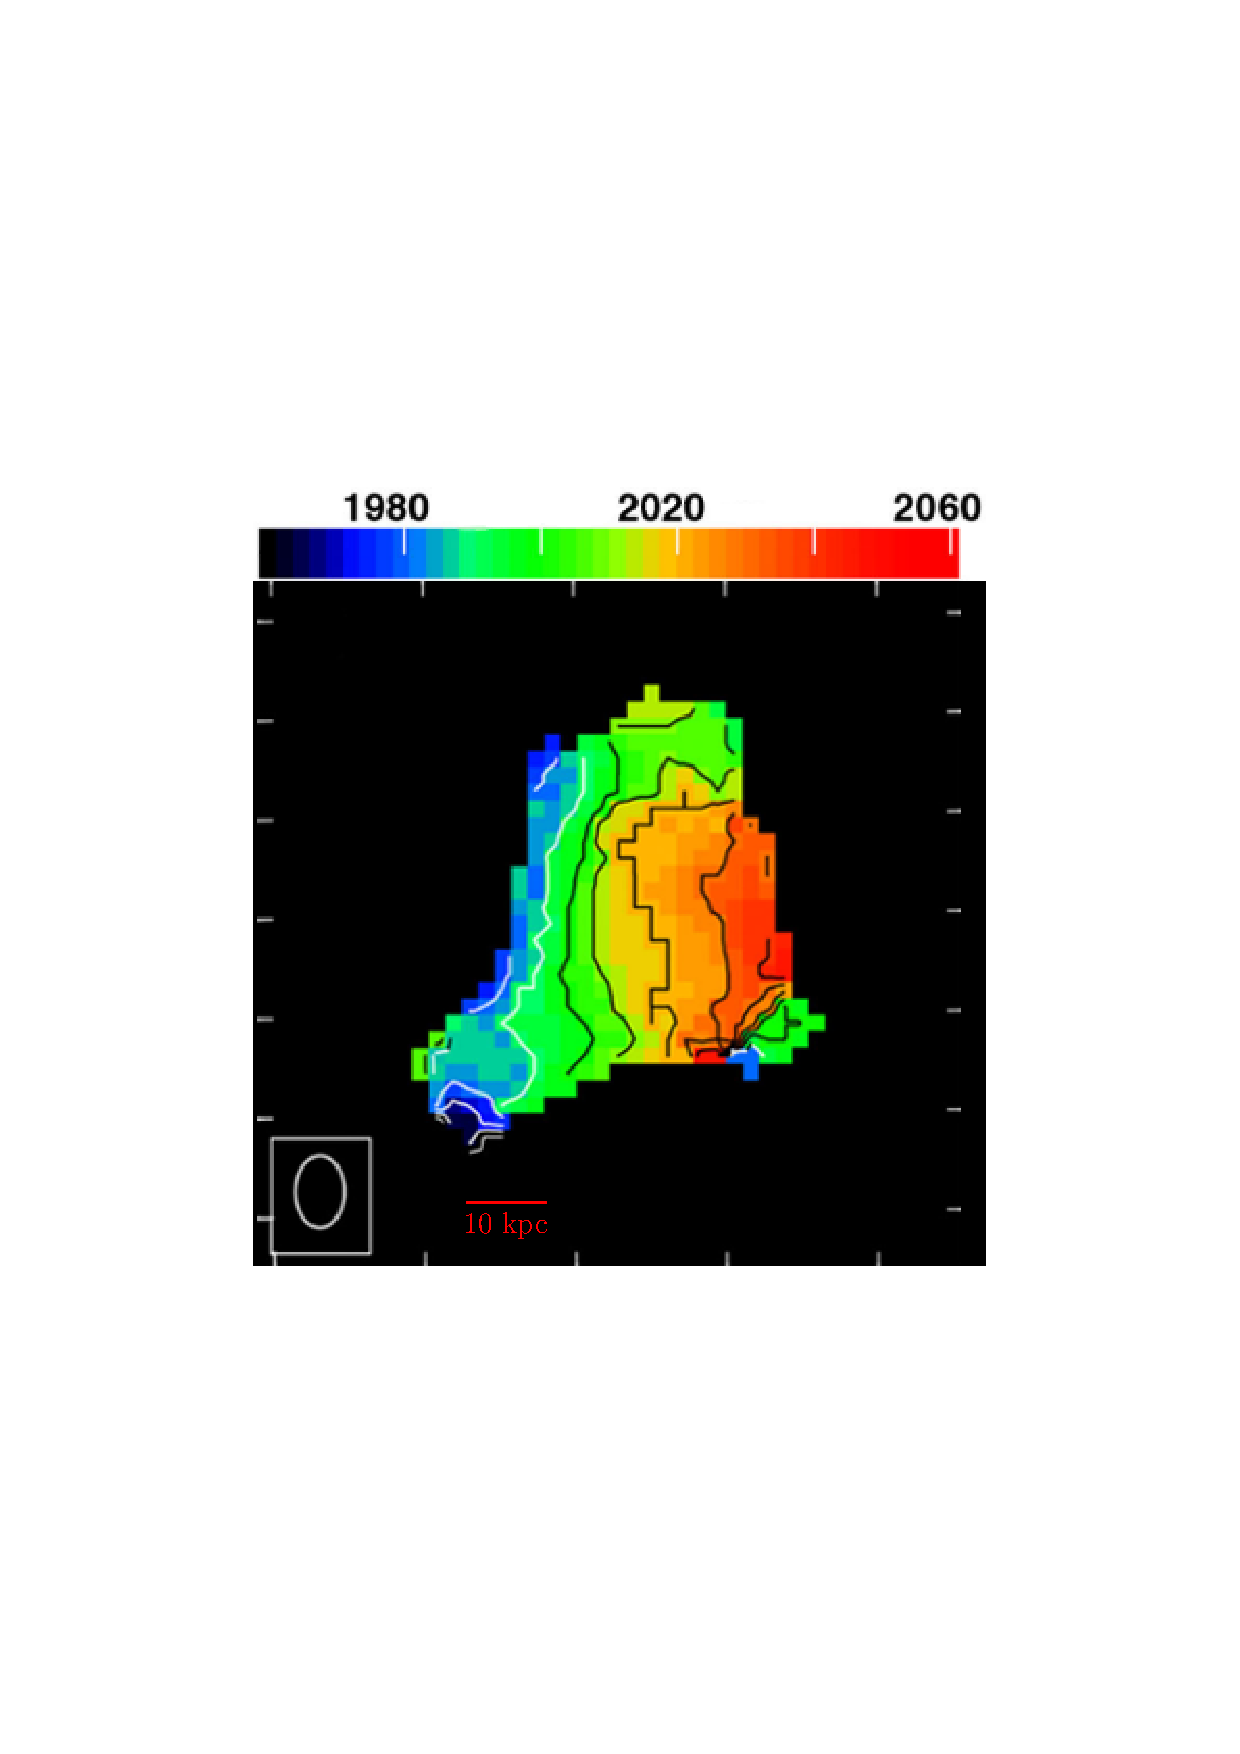
\includegraphics[width=0.9\textwidth]{NGC_LIKE/kin_scale.pdf}\\[3ex]
  \caption{}
  \label{fig:hi_kin}
\end{subfigure}
\begin{subfigure}[b]{0.6\textwidth}
  \centering
  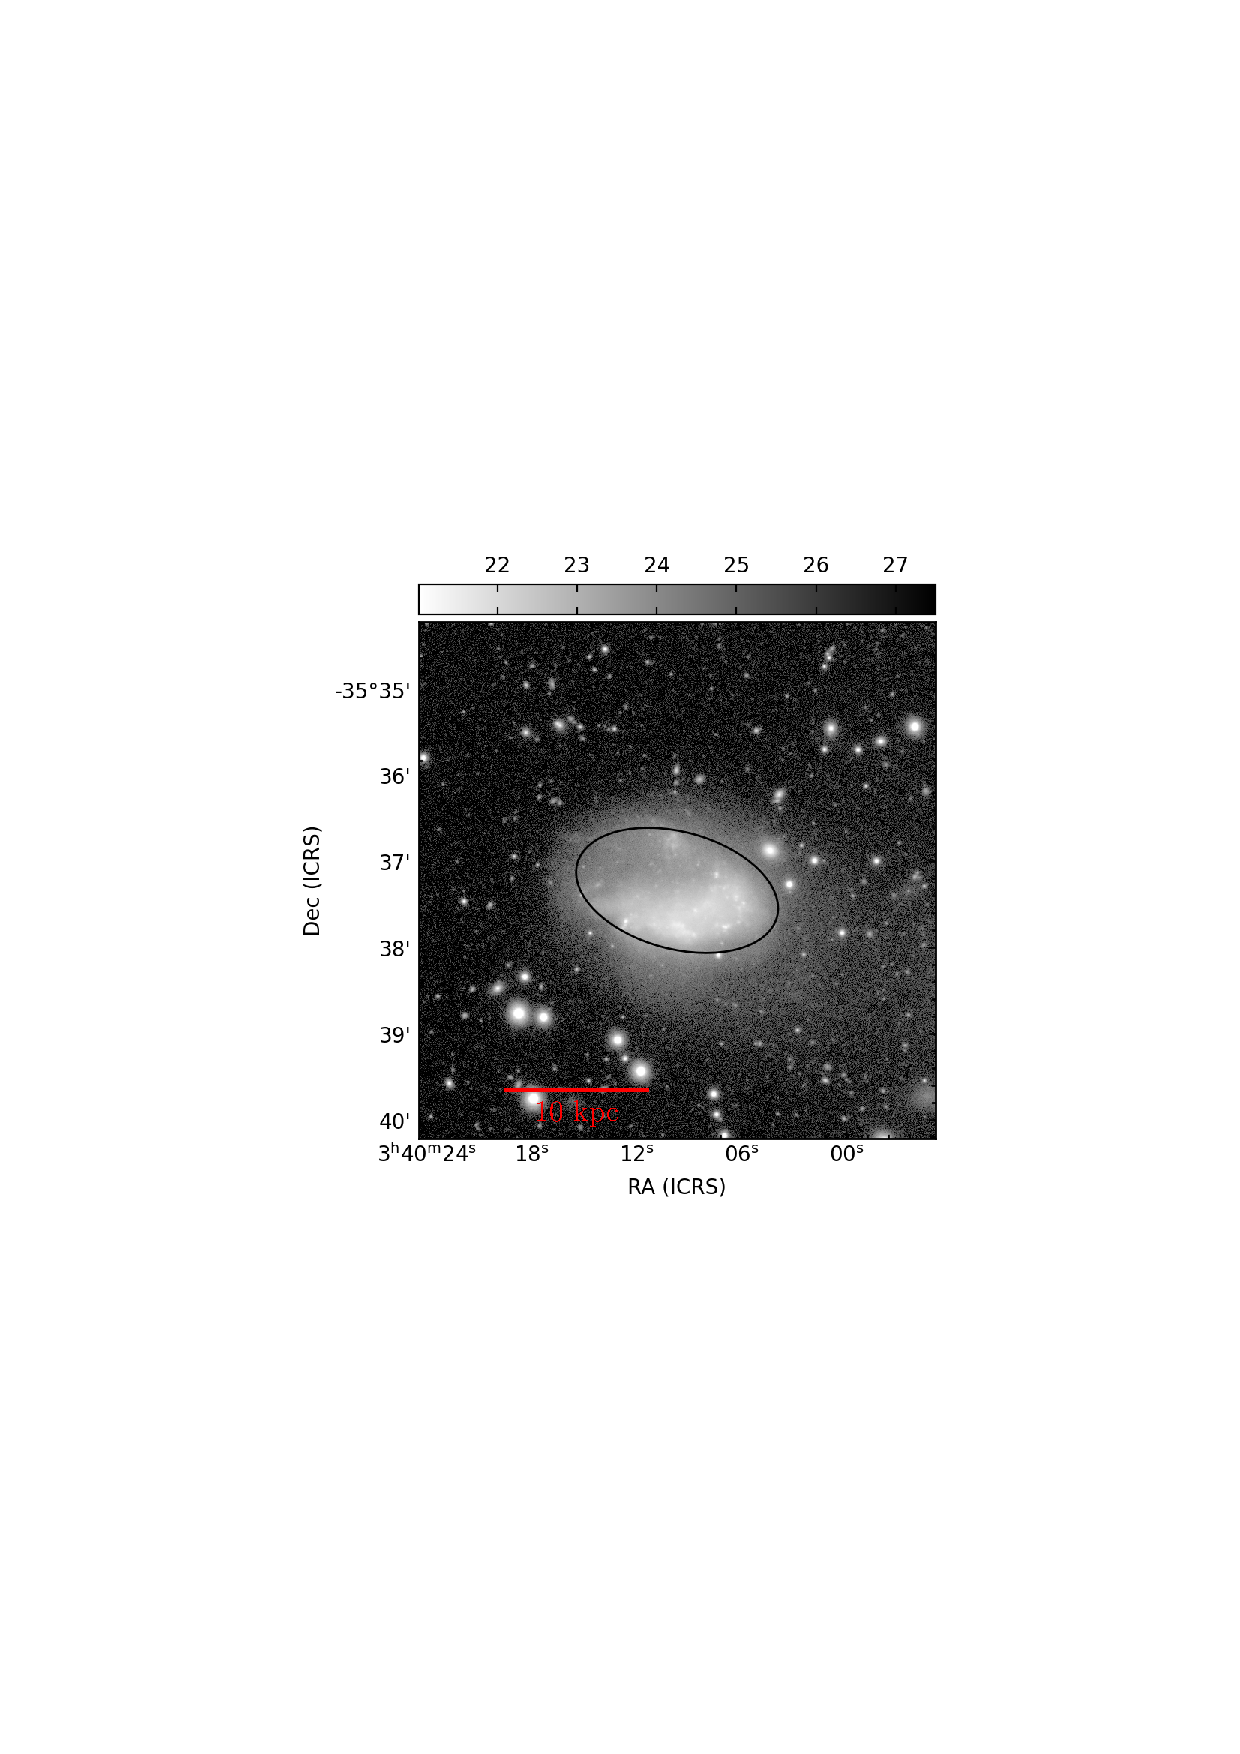
\includegraphics[width=\textwidth]{NGC_LIKE/ngc_tide_scale.pdf}%\\[3ex]
  \caption{}
  \label{fig:r_band}
\end{subfigure}
% \hfill
\caption{
Images of NGC~1427A from \citet{Lee-Waddell2018} for illustrative purposes:~(a) VST image with overplotted in red contours of constant \Hi{} column density at levels $(0.5, 1, 2, 5, 10) \times 10^{20}$~amu~cm$^{-2}$;
(b) gas kinematics (recessional velocity in km/s)
(c) $r'$-band image (in mag/arcsec$^2$).
A length scale at the assumed cluster distance is indicated in red.}
\label{fig:NGC_OBSERVATIONS}
\end{figure*}
NGC 1427A is a gas-rich dwarf irregular galaxy in the Fornax Cluster.
Recessional velocity measurements indicate that NGC~1427A is moving with a line-of-sight velocity of around 2028 km/s \citep{Bureau1996, Schroder2001}.
Accordingly, if we assume NGC~1399 to be the cluster center, NGC~1427A travels away from us at a projected speed of around 700~km/s relative to the cluster center. NGC 1427A has a projected distance of 137 kpc from NGC1399\footnote{The angular separation is 1373$\arcsec$ = 137~kpc, throughout the paper, we assume a fiducial distance of the cluster center of 20~Mpc.}.

A false-colour HST image of the galaxy is shown in Figure~\ref{fig:NGC1427A}.
The inset of Figure \ref{fig:NGC1427A} zooms in on the Northern Clump, showing it to be composed of two loose stellar clusters with embedded \Hii{} regions.
The Northern Clump also appears to be connected to the north-west rim of NGC~1427A's main body via a tenuous stream of stars.
The directions of the \Hi{} tail and towards the Fornax Cluster center are indicated with arrows.
The dotted ellipse is the same as in Figures 1 and 2 of \citet{Lee-Waddell2018} and indicates the shape and direction of the faint outskirts of the galaxy.
We interpret these low-surface-brightness stellar features, which point towards the north-east and south-west (effectively captured by the ellipses in Figure~\ref{fig:NGC1427A} and \ref{fig:r_band}), are quite distinct from the much brighter inner regions of the galaxy's main body, as tidal features.
The Northern Clump, which we discuss in detail in Section~\ref{NC1427A}, may be associated with these tidal features.

\citet{Chaname2000} presents a lower limit for the dynamical mass of NGC~1427A using a rigid-body rotation model: $M_{\mathrm{dyn}}~>~(9\pm 3)\times 10^9 M_\odot$.
Following the calibrated empirical relation of \citet{Taylor2011}, the stellar mass estimated by \citet{Lee-Waddell2018} is $M_{\star} \approx 10^9 M_\odot$ while its total \Hi{} mass is determined to be $M_{\mathrm HI} = (2.1 \pm 0.2) \times 10^9 M_\odot$.
The galaxy has a conspicuous \Hi{} tail, containing about $10$ per cent of all \Hi{} gas in NGC~1427A, pointing towards the south-east as well as stellar tidal extensions along a north-east to south-west axis.
In other words:~the gaseous and stellar extensions are almost perpendicular to each other.
NGC~1427A was not detected in CO emission, providing an upper limit on its molecular gas mass of the order of $M_{\mathrm H_{2}}~\sim 10^8$~M$_\odot$ \citep{Zabel2019}. These authors report the detection of a single 3~mm continuum source without an optical counterpart but its nature remains unclear.
A distinct young stellar clump is visible in the northern rim of the galaxy.
On high-resolution images, this clump, the rim, as well as the galaxy's main stellar body are resolved into many individual OB associations and clusters, some with accompanying H$\alpha$-emission \citep{Hilker1997, Sivanandam2014}.
Clearly, star formation proceeds in many dispersed small bursts.

Various hypotheses regarding the evolution of NGC 1427A, and especially its extraordinary configuration of tails, have been proposed.
These include recent interactions with other nearby galaxies \citep{Cellone1997}, a merger with an object that now forms the northern stellar clump \citep{Lee-Waddell2018},
the tidal interaction with the cluster potential, and ram-pressure stripping of its gas by the cluster hot gas halo \citep{Chaname2000, Mora2015}.
%This galaxy has been described by \citet{Laustesen1987} with this expression \emph{"It contains a large number of gaseous and luminous clusters, which partially form a ring towards the western edge of the galaxy”}. \citep{Cellone1997}
%What \sven{is especially striking} regarding NGC 1427A is the relative direction of its twin stellar and gaseous tails\sven{:~they are almost perpendicular to each other}.
% Various hypothesis on the formation scenarios have been proposed \cite{Hilker1997, Cellone1997, Chaname2000, Mora2015, Lee-Waddell2018}:
% tidal interactions with other nearby galaxies, tidal interaction with the cluster potential and ram pressure stripping of its gas by the cluster hot gas halo.

To try and identify the environmental processes acting on NGC~1427A, we first selected those properties of this dwarf galaxy that were most likely to be indicative of those processes and not of internal effects. Those are:
\begin{enumerate}
    \item the direction towards the Fornax cluster centrum,
    \item the direction of the axis of the stellar tidal extension,
    \item the direction of the \Hi{} tail.
\end{enumerate}
These parameters are most tightly linked with NGC~1427A's orbit through the Fornax Cluster and are expected to be relatively insensitive to the accidents and vagaries of its evolution before its acquisition by the cluster.

Thus, our analysis differs from that of \citet{Lee-Waddell2018} where the ram-pressure hypothesis is discussed based on stellar colour and galaxy morphology information.
Their new data indeed rule out a ram pressure origin for the optical appearance of the galaxy, but they leave open the question whether ram pressure may have played a role in the formation of the \Hi{} tail.

% We carried out a morphological search throughout our suite of simulations to isolate snapshots with the above properties respecting.% which can be useful to characterise the effects leading to such peculiar morphology.
% We found that the main effects generating peculiar morphology are indeed the combination of galaxy rotation, ram pressure and tidal interaction close to the cluster center.
% % It's clear also (see Figure \ref{fig:3dview}) that gaseous and stellar components react differently to the main stretching factors: ram pressure and gravity gradient.

% Instead, we take verbatim the indication from the \Hi{} map (their Figure 3): \emph{the neutral hydrogen galactic tail is a direct indication of the direction of motion of the galaxy}.
% Moreover, the \Hi{} velocity distribution as measured by \citet{Lee-Waddell2018} shows that the \Hi{} tail in its west part is receding more than the eastward part.
% As opposed to a rotation, we interpret the \Hi{} LOS velocity gradient as a direct indication of the stripping process. % \Hi{} 21 line profiles in \cite[p.63]{Bureau1996} do not show a double horn profile.



% \todo{
% % Possible bibliographic items to take into account: \citet{Bournaud2004}

% Simulation related bibliographic items to take into account: \cite{Joshi2018, Joshi2020}
% }

% \section{Observations}
% \cite{Lee-Waddell2018}
% SFR = 0.065 \Msun yr$^{-1}$ and $\log$(sSFR) = -10 from \cite{Sivanandam2014}
% \begin{figure}
% 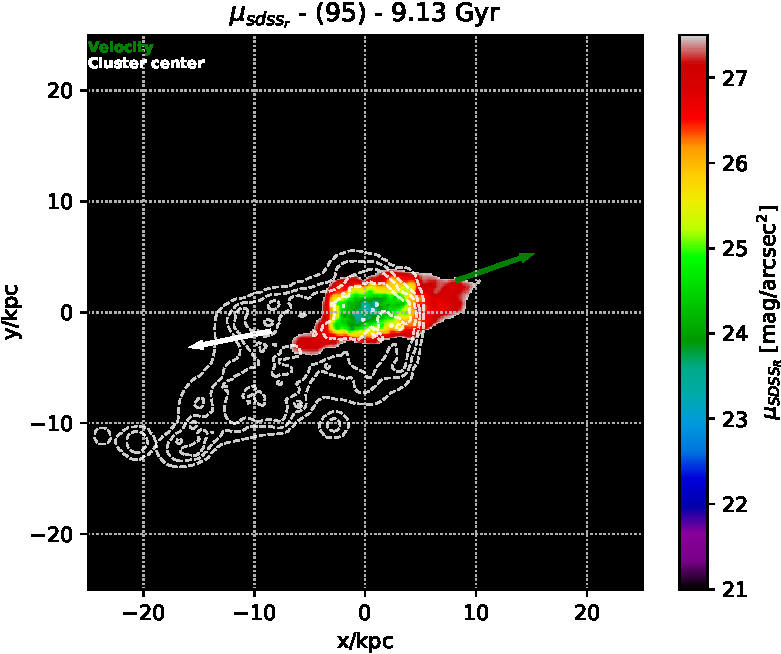
\includegraphics[width=\columnwidth]{69p100_0095_sb-crop.pdf}
% \caption{Surface brightness map with superimposed \Hi{} density contours with 5 equidistant in log-scale levels from $10^{17}$ to $10^{22}$ atoms/cm$^2$.}
% \label{fig:sb}
% \end{figure}

\section{Simulations} \label{sec:simulations}
\begin{figure}
\centering
\begin{subfigure}[b]{0.49\textwidth}
 \centering
 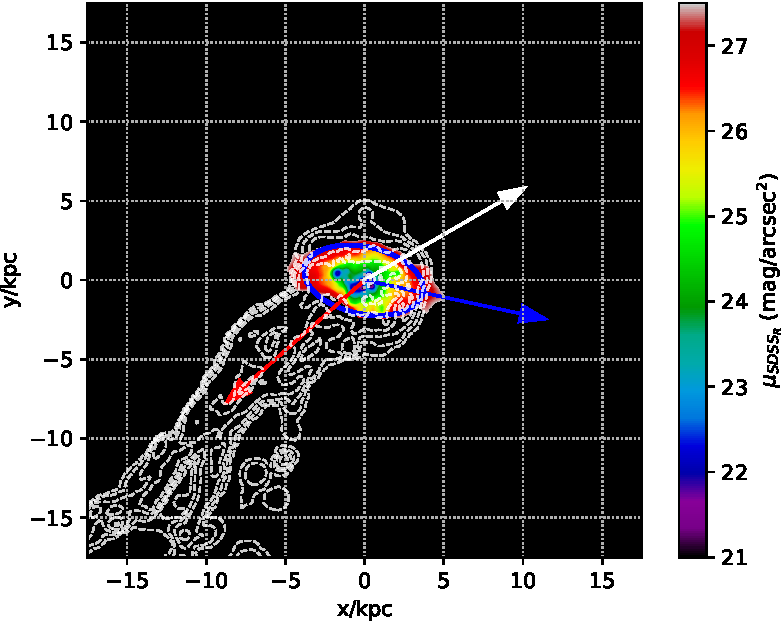
\includegraphics[width=\textwidth]{NGC_LIKE/SB.pdf}
 \caption{}
 \label{fig:sb_arrows}
\end{subfigure}
 \hfill
  \begin{subfigure}[b]{0.5\textwidth}
  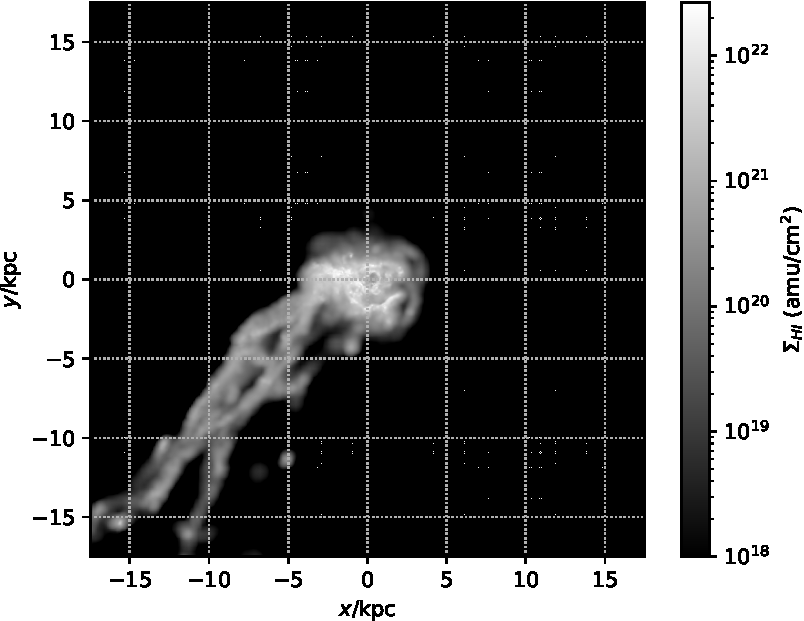
\includegraphics[width=\textwidth]{NGC_LIKE/HI.pdf}
  \caption{}
  \label{fig:sim_hi_density}
\end{subfigure}
\hfill
\begin{subfigure}[b]{0.5\textwidth}
  \centering
  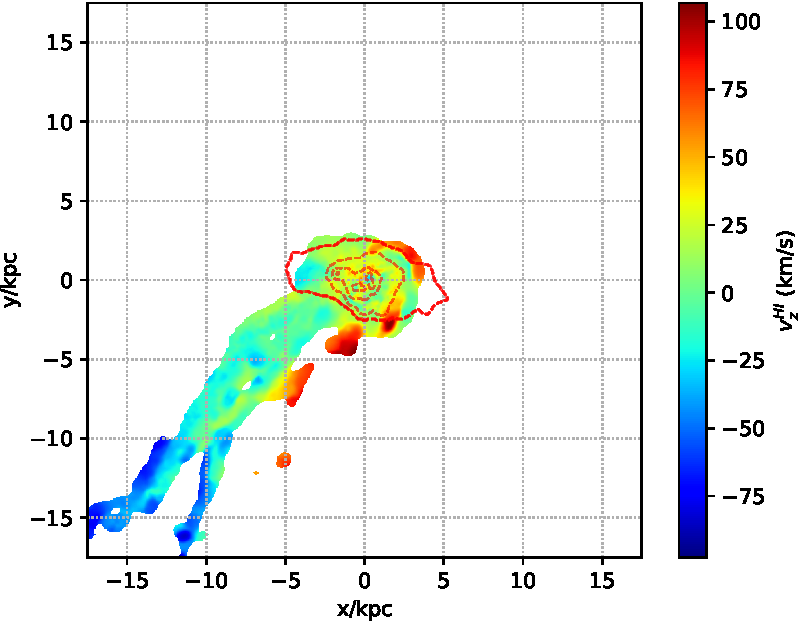
\includegraphics[width=\textwidth]{NGC_LIKE/HI_VEL.pdf}
  \caption{}
  \label{fig:sim_hi_kin}
\end{subfigure}
 \vfill
\caption{A simulation snapshot (ID 68, see Table \ref{tbl:sim}) on an orbit with 100 kpc pericenter distance, showing stellar tidal and gaseous stripped tails.
(a) $r'$-band surface brightness with \Hi{} column density contours as seen from a point of view for which the projected cluster-centric distance $r_p = 77$ kpc and the recessional velocity $-793$ km/s.
\Hi{} contours are drawn at column density levels [$10^{17}, 10^{18}, 10^{19}, 10^{20}, 10^{21}$]~amu~cm$^{-2}$. The white arrow points towards the cluster center, whereas the blue and the red arrows are the computed orientation of the stellar tail and the gaseous tail respectively, see Section \ref{sec:morphological_quest}.
%(same as \citet{Lee-Waddell2018})
(b) The column density of the neutral hydrogen, highlighting clumpy blobs of stripped \Hi{}.
(c) SPH map of the \Hi{} velocity field where the \Hi{} tail in its rightmost part is receding more than the more detached part.
For reference, the [22, 24, 26, 28]~mag/arcsec$^2$ isophotes are shown as dashed red contours.
We stress that our Fornax cluster dwarf galaxy simulations were not designed to reproduce all the details of this particular galaxy. Nonetheless, remarkable similarities can be found.}

\label{fig:selected_snapshot}
\end{figure}

The simulations used in this chapter are described in full details in \refsec{sec:fornax_sim}.
We stress that they have not been set up to mimic NGC~1427A in any particular way. Therefore, not all details can be expected to exactly match with observations.
Nonetheless, these simulations provide valuable insights not only into the phenomena at play but, more importantly, they can be used to infer the most likely current orbital phase of the galaxy.


\section{Constraining the orbital phase of NGC~1427A} \label{sec:results}

\subsection{Quantitative morphological search}
\label{sec:morphological_quest}

We carried out a systematic search among all the simulation snapshots, portraying different dwarfs at different times on different orbits.
We observed each snapshot from different points of view in order to select the snapshots and their orientation most resembling the observed galaxy using four measurable quantities:
\begin{enumerate}
    \item[(i)] the projected cluster-centric distance, $r_p$;
    \item[(ii)] the line-of-sight velocity with respect to the cluster center,~$v_p$;
    \item[(iii)] the position angle of the outer isophotes, quantified as the angle $\alpha$ between the projected cluster center direction and the direction of the $26.5$~mag/arcsec$^2$ isophote in $r'$ band, see Figure~\ref{fig:angles_scheme};
    \item[(iv)] the orientation of the \Hi{} tail as measured with the angle $\beta$ between the isophote orientation and the direction of the highest variance of the image obtained by computing the second order moments of the \Hi{} SPH map \citep{Stobie1980}.
\end{enumerate}
\begin{figure}
\centering
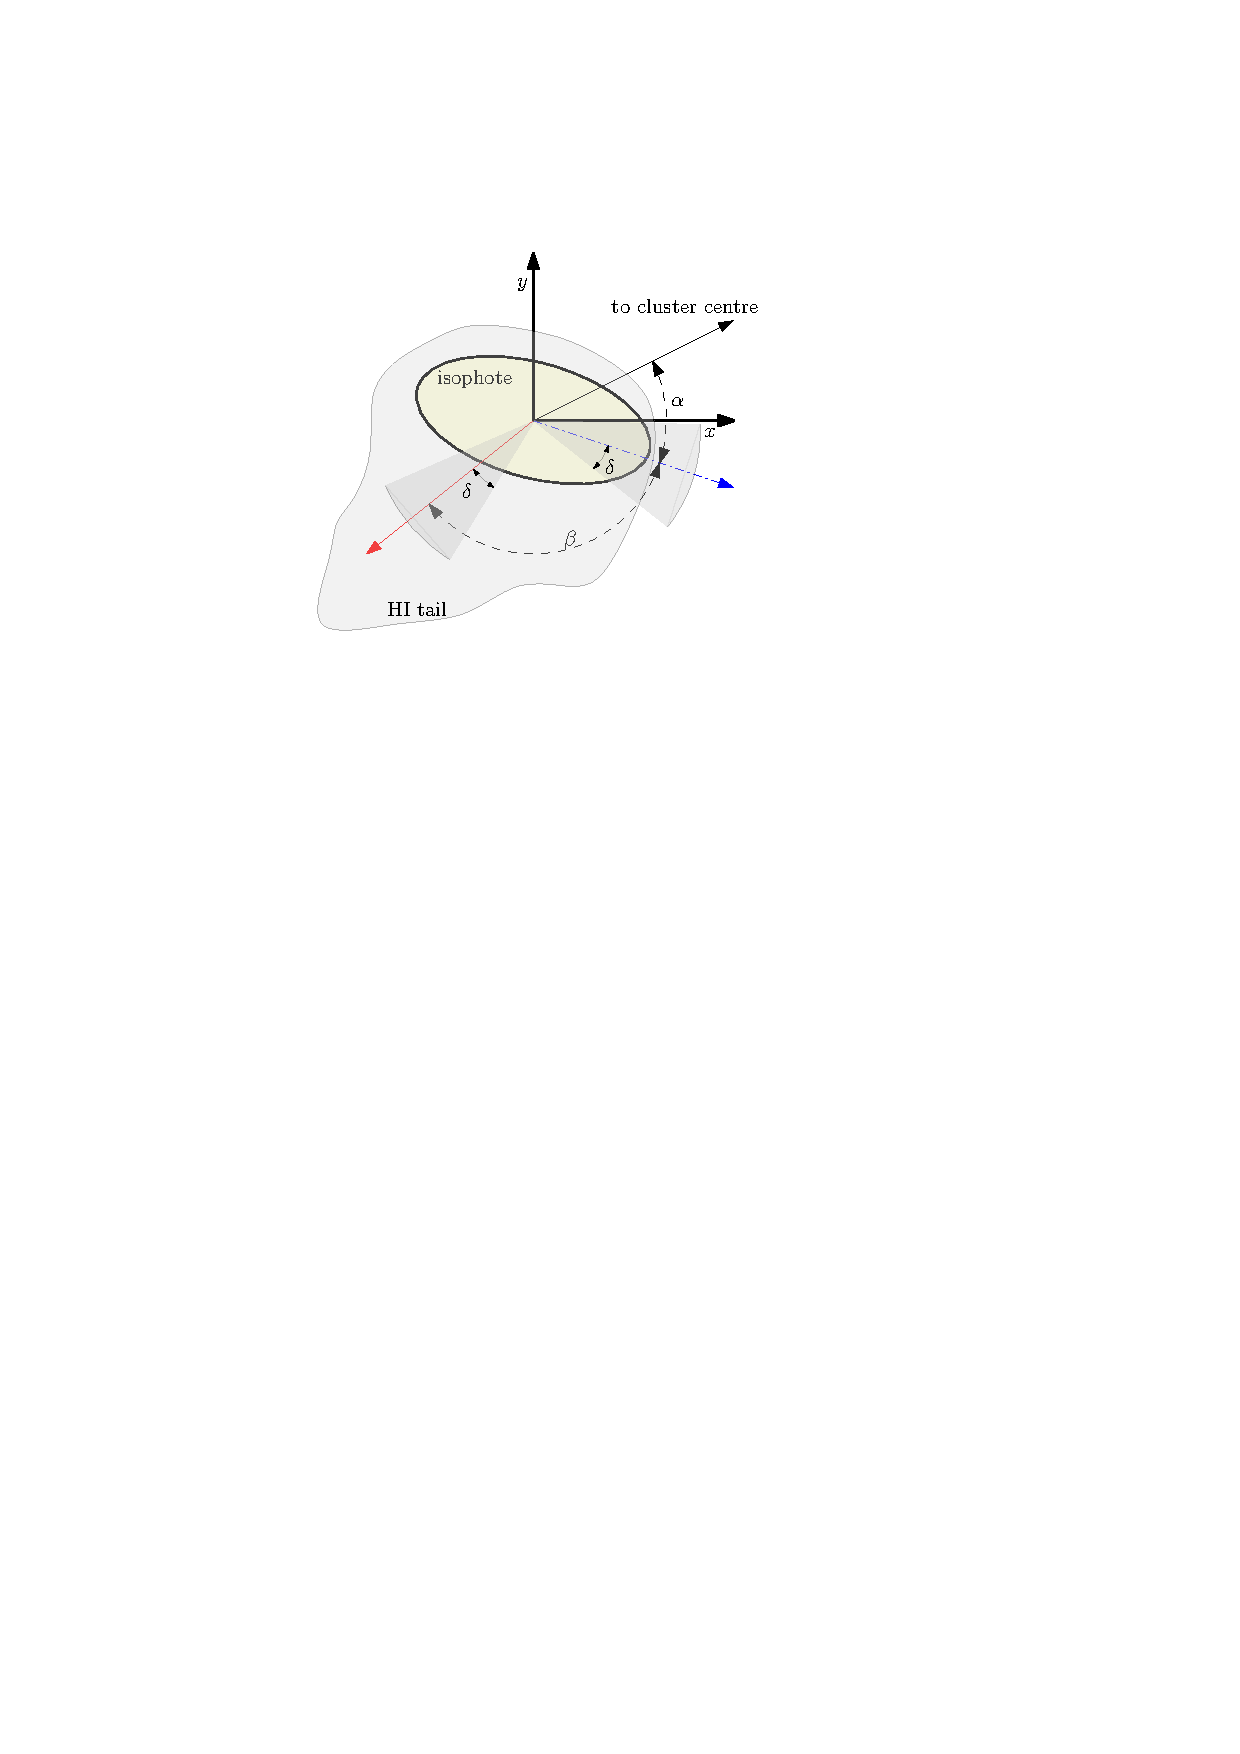
\includegraphics[width=0.65\columnwidth]{alpha_beta_coloured_for_fig.pdf}
\caption{Angles $\alpha, \beta$ definitions used to set up the  requirements for the morphological search. $\delta$ is the angle tolerance used for the selection. Blue and red arrows are defined as in Figure \ref{fig:sb_arrows}. Darker grey shaded regions are the allowed directions of the oriented snapshots tidal stellar tail and \Hi{} tail.}
\label{fig:angles_scheme}
\end{figure}
\begin{figure}
\centering
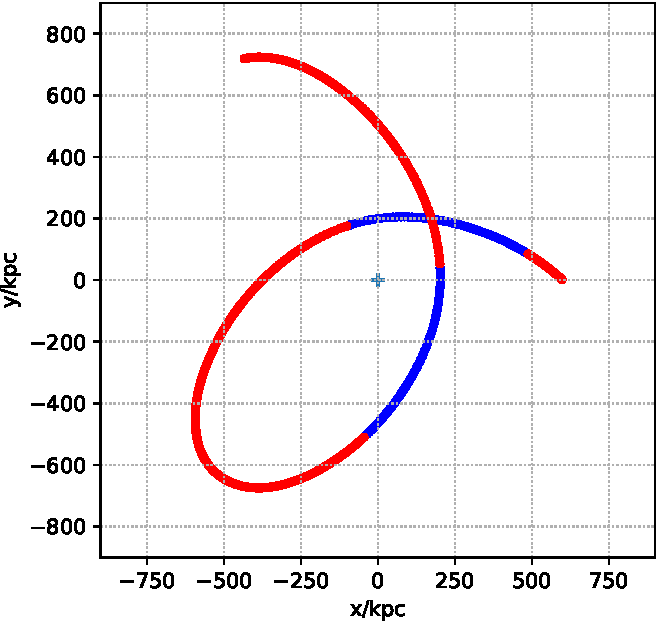
\includegraphics[width=0.55\columnwidth]{good_traj.pdf}
\caption{A trajectory with pericenter of 200~kpc. In blue the orbital phases for which there are snapshots with projected distance and recessional velocity compatible with the ones of NGC~1427A (i.e. snapshots fulfilling requirements (i)-(ii)) for some points of view.
In this case $r_p = 137$~kpc, $v_p = -693$~km/s.}
\label{fig:good_traj}
\end{figure}
We highlight that the search has been carried out using only morphological and orbital parameters, given our focus on the peculiar morphology of NGC~1427A.
Moreover, the criteria used to compare simulations to observations are the ones that best represent the effects of the cluster environment: the relative directions of the tidal pull and the ram pressure stripping. Indeed, the first two requirements put constraints on the orbital position and hence on the orbital phase of the simulated dwarf. The latter two require that the isophotal tail and the neutral gas tail are oriented as in NGC~1427A.
By selecting a faint isophote for criterion (iii) we are tracing the outer tidal extensions of the stellar body.
Inspection of the evolution of the direction of the principal axes of the stellar density distribution along a simulated dwarf galaxy's orbit shows that the galaxy outskirts rapidly forget their initial spatial orientation and become strongly aligned with the cluster center around pericenter and apocenter. On the inward or outbound legs of a galaxy's orbit, this elongation occurs parallel with its orbital velocity. This evidence for a tight correlation between a dwarf galaxy's elongation and its orbital phase, led us to include criterion (iii).

From VST images of \citet[][]{Lee-Waddell2018} \citep[originally from the deep survey presented in][]{Iodice2016} we used the position angle of 15~deg of the fitted ellipse in its Figure 2.
From the \Hi{} maps of Figures 1 and 3 of the same paper (see Figures \ref{fig:hi_contours} and \ref{fig:hi_kin} above) we assumed an inclination of the \Hi{} tail of -135~deg (pointing south-east).
%, see Figure \ref{fig:arrows}.
Given that the direction of the cluster center is around 30~deg north-west, the resulting target angles are $\bar \alpha = 45$~deg, $\bar \beta = 120$ deg, as in Figure~\ref{fig:angles_scheme}.

For each snapshot, we started by finding the orbital phase which fulfils the first two requirements.
Each requirement is satisfied by the set of points of view constituting the generatrices of a cone centered on the galaxy position.
By intersecting two cones it is possible to find the points of view satisfying the requirements.
This is equivalent to solving a quadratic equation (see Section \ref{sec:cone_intersection}) whose two solutions are two points of view satisfying the requirements (i) and (ii).
Each snapshot is then rotated as if it was observed from the peculiar point of view yielding the imposed clustercentric distance and the recessional velocity.
The more radial the orbit is, the higher the number of suitable snapshots which will be further selected using requirements (iii) and (iv), see Figure \ref{fig:good_traj}.

With the assumed cluster center at a distance of 20~Mpc from us (see Section \ref{sec:observations}), we imposed as targets the two quantities $\bar r_p=137$~kpc and $\bar v_p=-693$~km/s with measures for NGC 1427A (the projected distance on the sky and recessional velocity of NGC~1427A relative to NGC~1399).
In order to take into account uncertainties in the measured $\bar r_p$ and $\bar v_p$ and to capture the sensitivity of the procedure to the selected projected distance and recessional velocity, we repeated the same procedure for each simulated snapshot but allowing for other slightly offset targets $r_p$ an $v_p$.
Practically, we fixed an offset in both quantities $r_p = \bar r_p \pm \Delta r$, $v_p = \bar v_p \pm \Delta v$ with $\Delta r = 100$ kpc, $\Delta v = 60$ km/s.
Also we added four other targets: $(\bar r_p \pm \Delta r, \bar v_p)$ and $(\bar r_p, \bar v_p \pm \Delta v)$ with same ($\Delta r, \Delta v$) as before.
Including the exact target $\bar r_p, \bar v_p$, at the end, we had nine targets to check for each snapshot.
In total, we obtained a dataset of 424,656 oriented snapshots.

For each snapshot surviving the selection of requirements (i) and (ii) and oriented so that $r_p$ and $v_p$ are the ones imposed, we created the surface brightness map and \Hi{} map.
We first fitted an ellipse to the contour corresponding to the $26.5$~mag/arcsec$^2$ isophote in $r'$ band.
We computed the second order moments of the \Hi{} map to obtain the direction of the neutral hydrogen tail.
Since we are interested in snapshots with an elongated \Hi{} tail in the South-East direction, we further selected only oriented snapshots with galactic projected velocity on the plane of the sky having a positive projection on the cluster center direction. This removes false positives with a \Hi{} tail inclined with the proper angle but extending towards the cluster center (from the image moments only the direction is returned, not the sense of elongation of the tail).
At the end of this pre-selection, we ended up with 59,896 oriented snapshots.

We then used requirements (iii) and (iv) to further refine the search.
In the following section we shall determine the distribution of the snapshots with tails similar to the observed galaxy using angles $\alpha$ and $\beta$, described above, and a tolerance $\delta$:
\begin{equation*}
\bar \alpha - \delta < \alpha < \bar \alpha + \delta, \qquad
\bar \beta - \delta < \beta < \bar \beta + \delta
\end{equation*}
The selection tolerance $\delta$ is then our main knob to filter-out snapshots oriented as NGC~1427A with angles $\bar \alpha$ and $\bar \beta$. The dependence of the results (and the number of oriented snapshots surviving the selection criteria (i-iv)) on its choice is quite strong, so in all the following histograms we highlight the $\delta$ chosen.


\subsection{Finding points of view - cones intersection}
\label{sec:cone_intersection}
Finding the point of views from which the galaxy appears as having the target projected clustercentric distance ($r_p$) and the proper line-of-sight velocity ($v_p$) is equivalent to solving the problem of intersecting two cones.

Given $\vec x$ the unit vector representing the direction of the point of view, and $\vec r$ and $\vec v$ the clustercentric position and velocity of the galaxy respectively, we can write the following conditions:

\begin{equation}
\label{eq:system}
\begin{cases}
\vec x \cdot \vec v = v_p\\
\vec x \cdot \vec r = \pm R\\
|\vec x|^2 = 1
\end{cases}
\end{equation}
where $R = \sqrt{r^2 -r_p^2}$. By using [$\vec r, \vec v, \vec r \times \vec v$] as basis (right-handed but not orthogonal), it is possible to express $\vec x$ as:
\begin{equation}
    \vec x = a \vec v + b \vec r + c ( \vec r \times \vec v).
\end{equation}
Substituting into \eqref{eq:system}:
\begin{equation}
\begin{cases}
a v^2 + b (\vec r \cdot \vec v) = v_p\\
a(\vec r \cdot \vec v) + b r^2 = \pm R\\
|\vec x|^2 = 1 = a v^2 + b r^2 + c^2 | \vec r \times \vec v|^2 + 2 ab(\vec r \cdot \vec v)
\end{cases}
\end{equation}
The last quadratic equation yields immediately two values of $c$ ($c_1$, $c_2$).

For each chosen sign of $R$, the system yields two solutions: ($\vec x_1$, $\vec x_2$) which can be used to rotate the galaxy snapshot as if it was seen from the directions $\vec x_1$ and  $\vec x_2$.

Each direction can be defined using two angles ($\varphi$ and $\theta$) representing the spherical coordinates of the unit vectors $\vec x_1$ and $\vec x_2$.

\begin{figure}
  \centering
  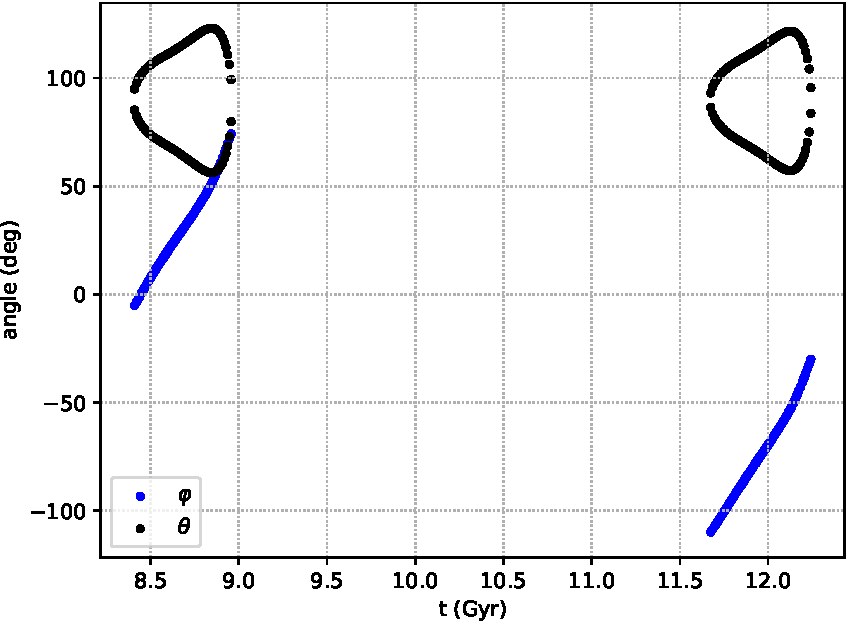
\includegraphics[width=0.8\columnwidth]{angles.pdf}
  \caption{Angles $\varphi, \theta$ defining the points of view of each snapshot of the trajectory of Figure \ref{fig:good_traj}. The angles are used to rotate the selected snapshots in order to obtain the target $r_p, v_p$. Only a subset of snapshots can be oriented to fulfil the requirements.}
  \label{fig:phitheta}
\end{figure}
In Figure \ref{fig:phitheta} an example of rotation angles for a particular simulated orbit is shown.
The angles $\varphi$ and $\theta$ are used to rotate the simulated galaxy as if it was observed from the peculiar point of view yielding the imposed clustercentric distance $r_p$ and the recessional velocity $v_p$.


\subsection{Distribution along the orbit of points of view satisfying the requirements}
\begin{figure}
\centering
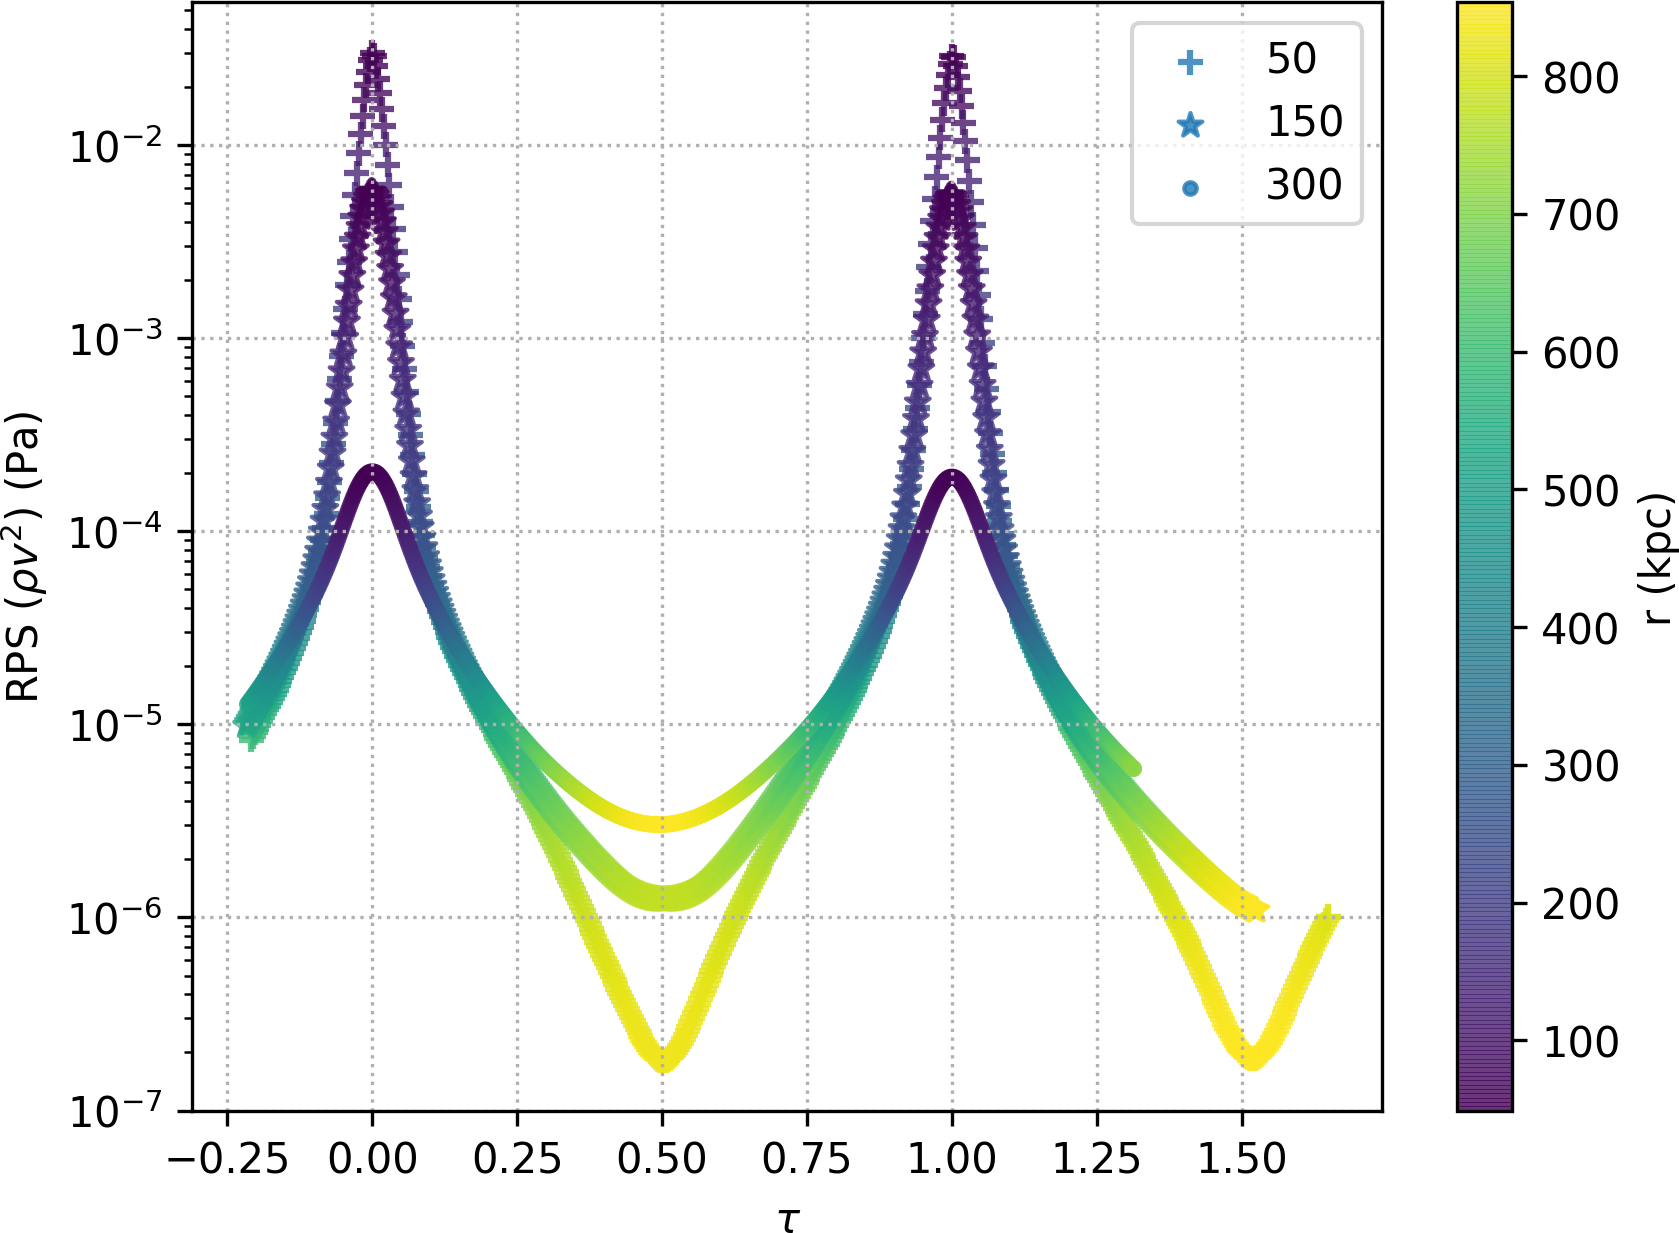
\includegraphics[width=0.8\columnwidth]{rps-crop.png}
\caption{The strength of the ram pressure ($\rho v^2$) as a function of normalised time $\tau$ (\cf{} equation \eqref{eq:tau}) for the ID 69 simulations on multiple orbits (orbit pericenter in kpc is indicated in the legend). The colour scales traces orbital distance with respect to the cluster center.}
\label{fig:r_rps}
\end{figure}
We computed the distribution of selected oriented snapshots with respect to the time from the pericenter passage.
We noted that all the snapshots surviving the selection are found within 200 Myr of a pericenter passage.

We ascertain the robustness of this result by varying the tolerance~$\delta$ of the comparison of the angles $\alpha, \beta$ with the observed ones.
Our orbital and morphological criteria are preferentially met by simulations with a stellar mass above $ \approx10^8 $ \Msun{}.
Less massive galaxies and galaxies on radial orbits are completely stripped from their HI gas, see Figure \ref{fig:m_hi}, because of the steep increase of ram pressure around pericenter as shown in Figure \ref{fig:r_rps}.
\begin{figure}
\centering
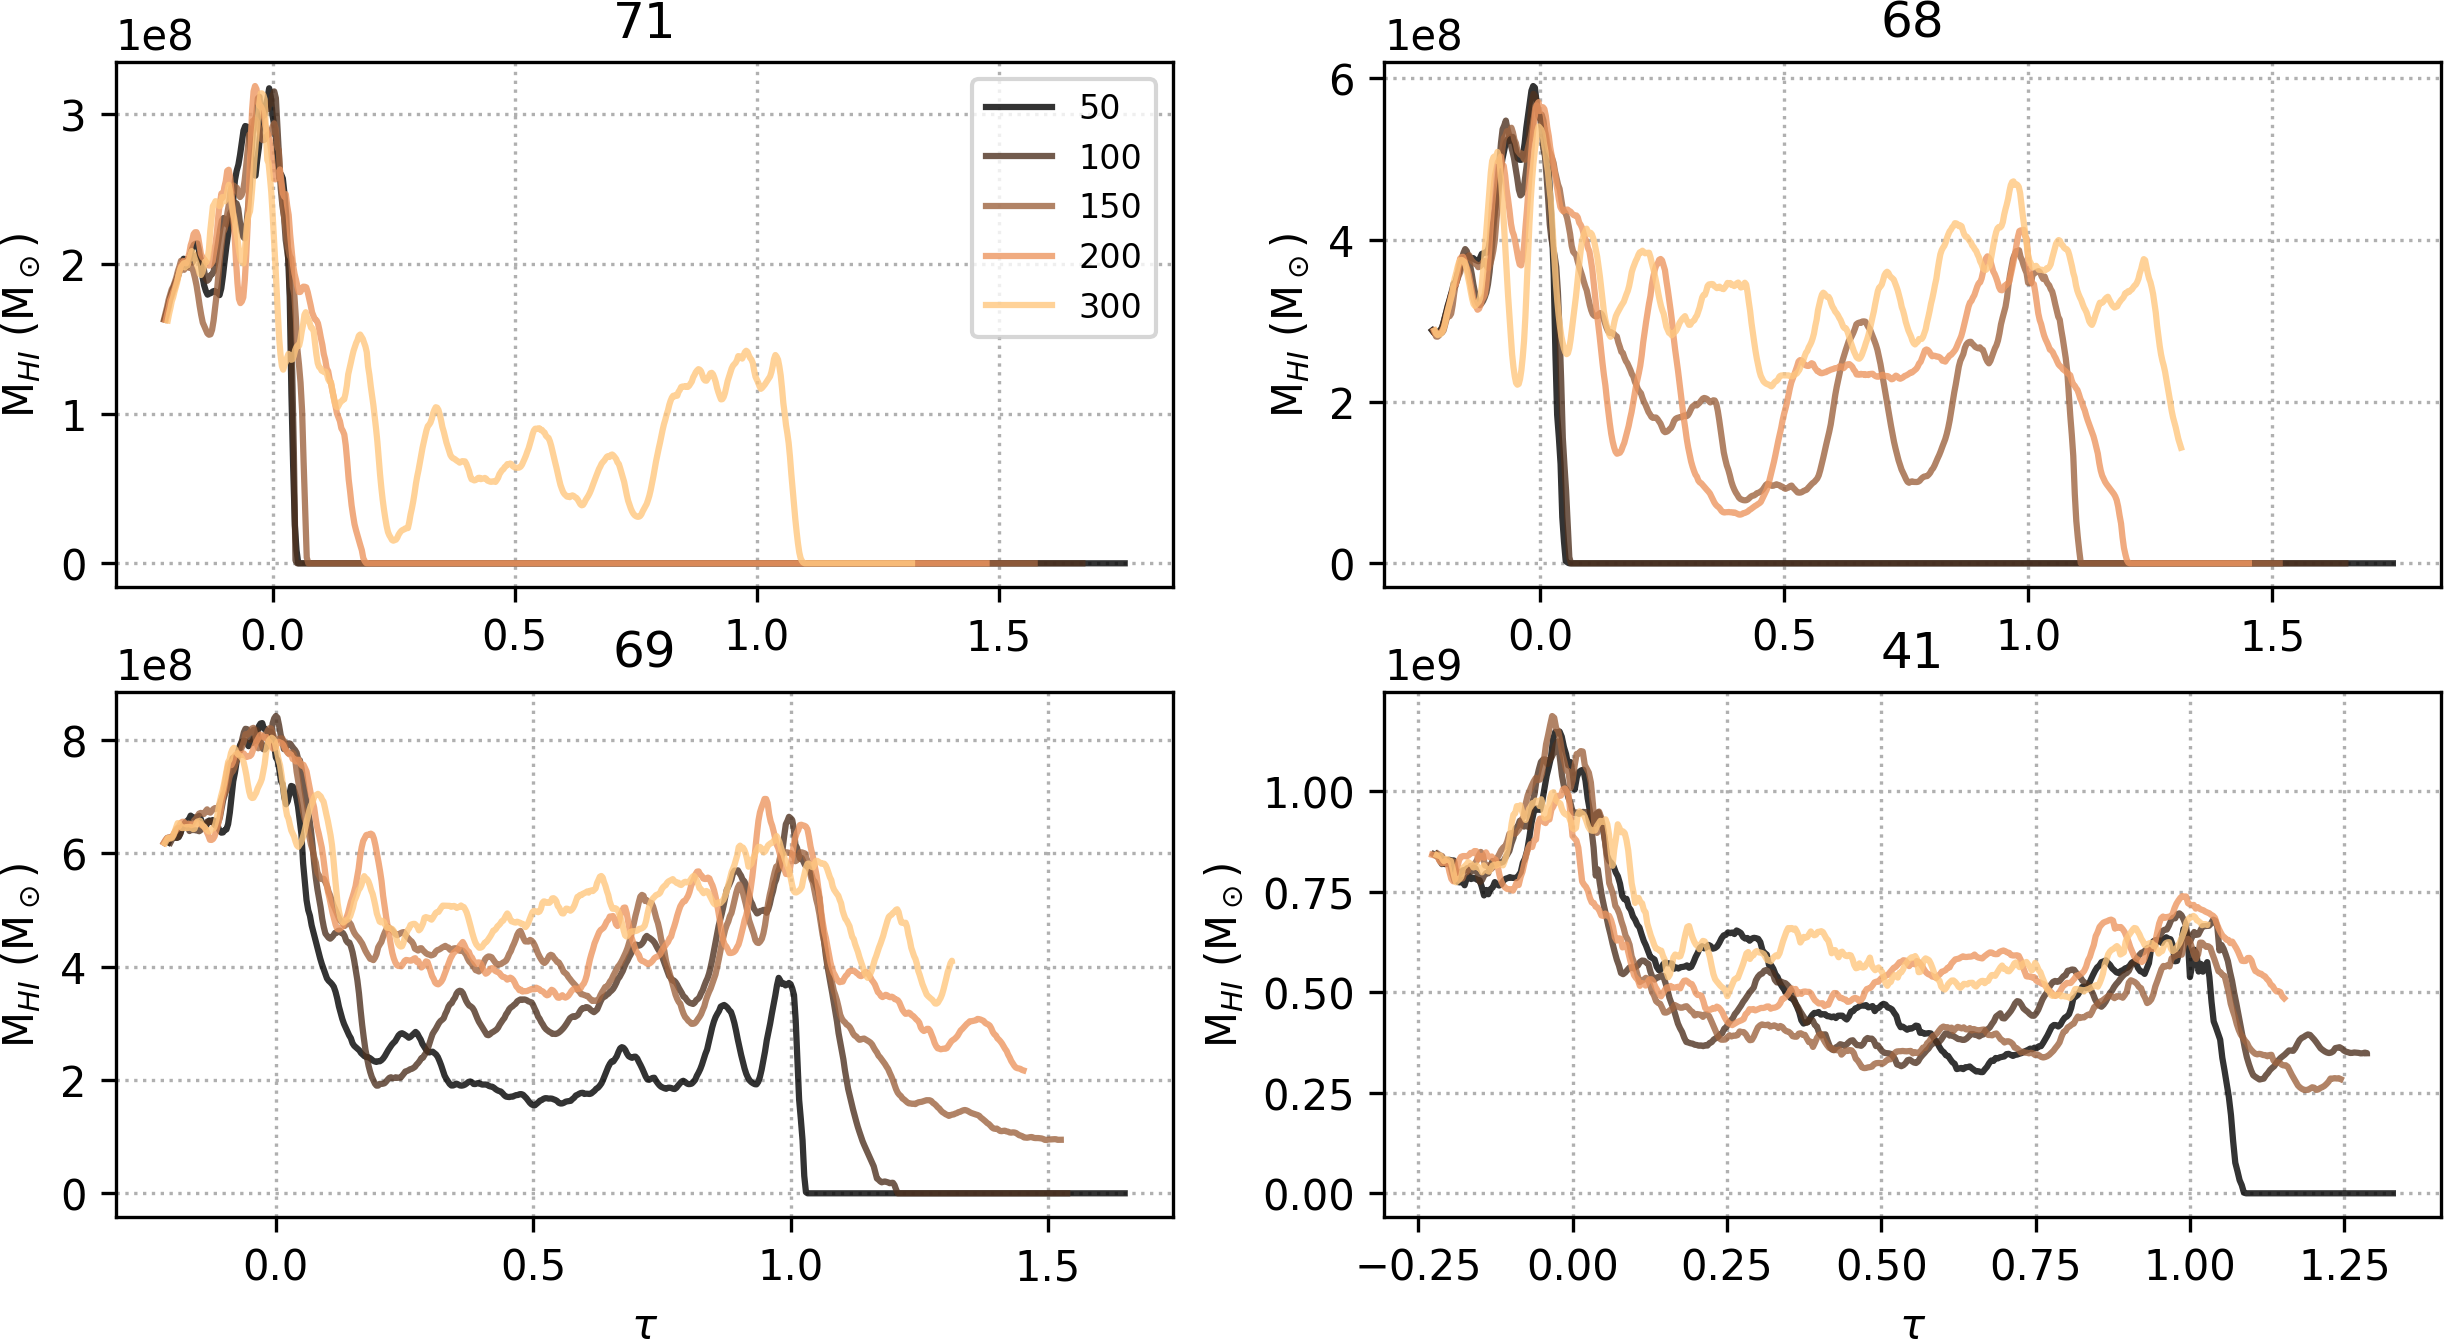
\includegraphics[width=\textwidth]{m_hi-crop.png}
\caption{Neutral gas mass as a function of normalised time $\tau$ as defined in equation \eqref{eq:tau}.
Each panel is labelled with the simulation ID (cf. Table~\ref{tbl:sim}) and contains information for the simulated dwarf launched on orbits with different pericenter distances (50, 100, 150, 200, 300 kpc identified by the colour legend in the top-left panel).
Gas is compressed when the isolated galaxy enters the cluster and as a consequence it cools down, thus increasing the neutral hydrogen mass.
Obviously, around pericenter, ram pressure stripping is effective at driving down the gas mass (as shown also in Figure~\ref{fig:r_rps}).
}
\label{fig:m_hi}
\end{figure}
Especially for radial orbits, no oriented snapshot is found on orbits of 50 and 100 kpc after first pericenter passage, regardless of the tolerance~$\delta$ considered, as shown in Figure~\ref{fig:histo_peri}.
For the most circular orbits, only snapshots undergoing second pericenter passage survive the selection. This is likely due to the first passage acting as `preprocessing' and making the galaxy potential shallow with higher chances to create tidal tails.
% \todo{I'm currently having a look at the distribution of ellipticity of the fitted isophotes to see how circular, and hence not so tidal, they are. Update: See figure noperi_all_stacked-crop.png }
In Figure~\ref{fig:histo_noperi} we performed the same analysis cumulatively counting all the oriented snapshots (without pericenter distance distinction) but using different isophotes.
The diagrams, even if noisier when using fainter isophotes, convey the same message: there is an abundance of correctly oriented snapshots (with tails as NGC~1427A) around first pericenter passage.
Indeed, tidal tails as those shown in Figure~\ref{fig:panel}, are present in low surface brightness regions of the dwarf, even if they are more difficult to measure.
The counterpart in NGC~1427A would be the faint stellar South-West elongation visible especially in $r'$-band, see Figure~\ref{fig:r_band}.

\begin{figure}
\centering
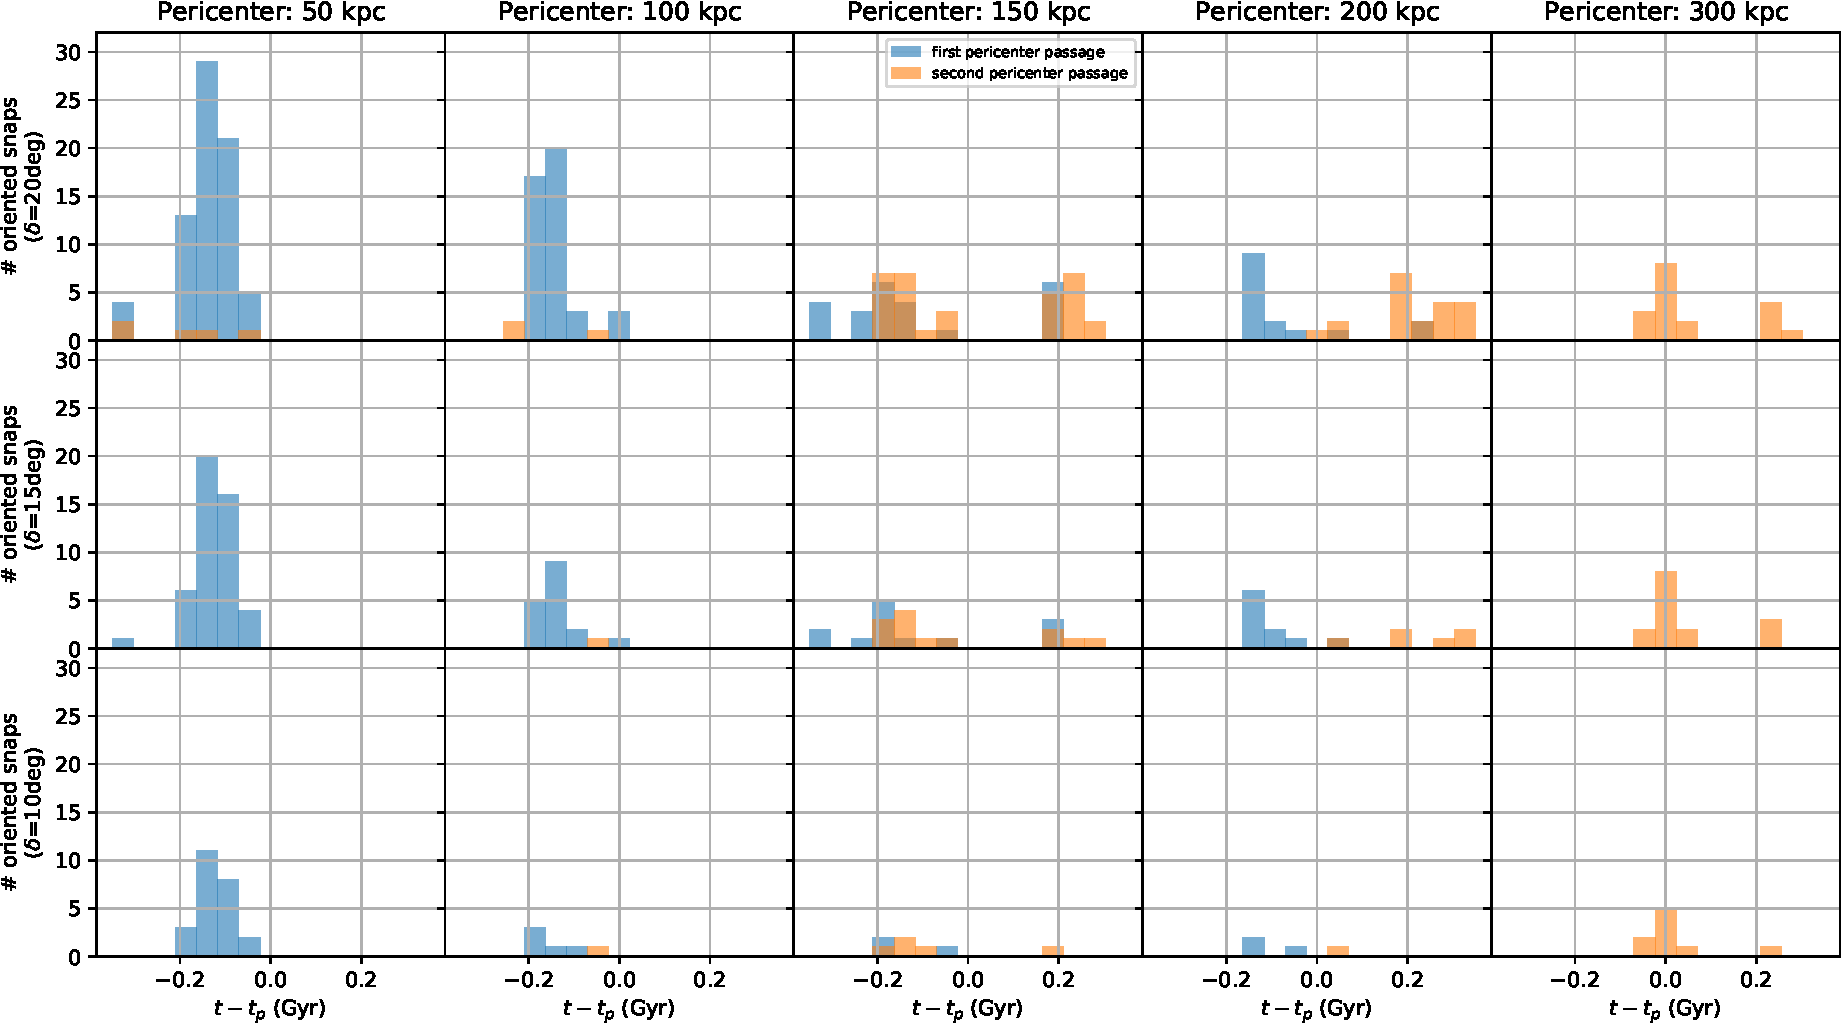
\includegraphics[width=\textwidth]{histo/histo_iso26.5_bins0.35-16.pdf}
\caption{Histograms of oriented snapshots fulfilling the requirements (i)-(iv), selected to be around first (blue) or second (orange) pericenter and grouped by orbital pericenter distances (50, 100, 150, 200, 300 kpc).
The isophote used to compute the stellar tail inclination is $26.5$~mag/arcsec$^2$ in $r'$ band.
The distribution is peaked at around 150 Myr before pericenter passage, especially in more radial orbits. The result is robust enough to be visible on stricter angle tolerances $\delta = [20, 15, 10]$~deg.
}
\label{fig:histo_peri}
\end{figure}

\begin{figure}
\centering
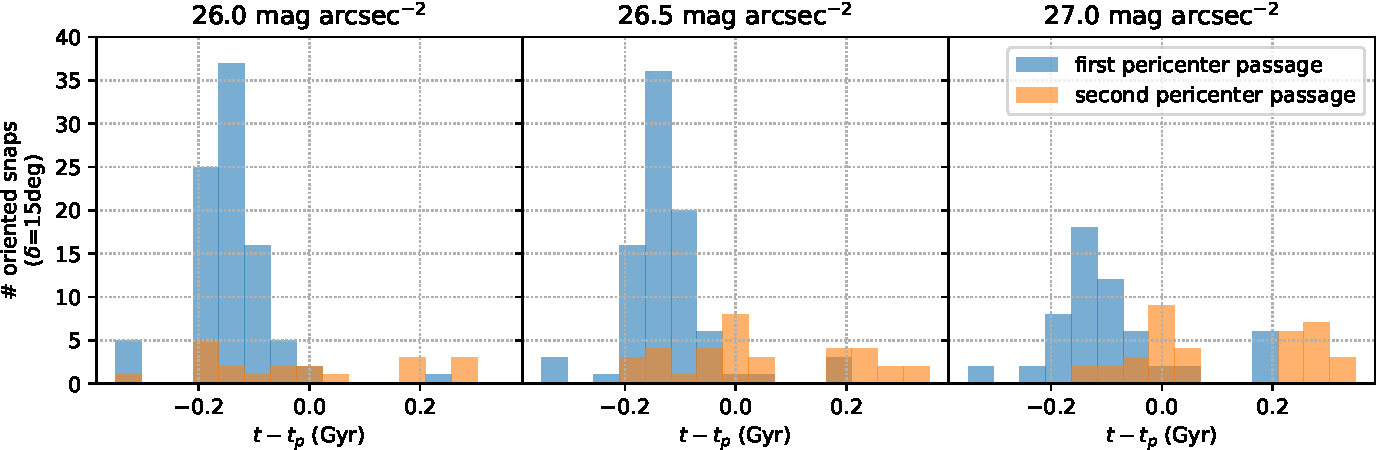
\includegraphics[width=\textwidth]{histo/iso_comparison_tol15_asym0.0_bins0.35-16.pdf}
\caption{Distribution in time relative to pericenter passage of oriented snapshots fulfilling the requirements (i)-(iv) with tolerance $\delta=15$ deg.
Histograms of selected snapshots are coloured relative to their orbital phase: around first (blue) or second (orange) pericenter.
Each column corresponds to a different isophote used to compute the stellar tidal orientation.
Irrespective of the isophote, the distribution remains peaked  around 150 Myr before pericenter passage.}
\label{fig:histo_noperi}
\end{figure}

\subsection{3D position of the galaxy in the Fornax context}

Based on the above described model, we can produce a quantitative estimation of the galaxy projected radial distance. This measure is actually a testable prediction with distance observations.
Unfortunately, current uncertainties on the distance measurements do not allow to unequivocally assess the position of the galaxy to be in front or behind the cluster center \citep{Georgiev2006}.

Using our models we can see which is the most likely radial distance relative to the cluster center of a galaxy with morphological features like NGC~1427A.
As shown in Figure \ref{fig:distance_prediction}, the preferred line of sight distance is around 200~kpc in front of the cluster center.

It is also possible to compute the flight angle $\gamma$ of the galaxy with respect to the line of sight direction (see Figure \ref{fig:gamma}).
As shown in Figure \ref{fig:velocity_prediction}, from the above models, the most frequent is $\gamma\approx 50$~deg.
Given that the stripped gaseous tail approximately follows the opposite direction of flight, measuring the flight angle in simulations can be useful to assess the real length of the gaseous tail in observations.
Our result would indicate the real tail to be roughly a factor 1.3 longer than the projected one.

\begin{figure}
\centering
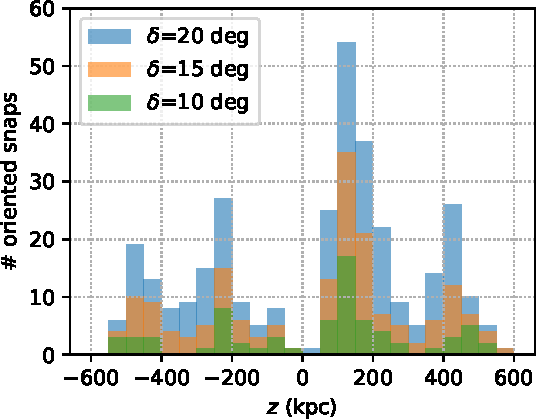
\includegraphics[width=0.8\columnwidth]{histo/multi_tol_dist_gauss_bins600_25.pdf}
\caption{Distribution of selected oriented snapshots with multiple tolerance $\delta$ along the projected line of sight. The zero point is 20~Mpc, assumed distance of NGC~1399. Positive values mean the galaxy being \emph{in front of} the cluster center.
%Overplotted a Kernel Desity Estimation for the distribution.
}
\label{fig:distance_prediction}
\end{figure}

\begin{figure}
\centering
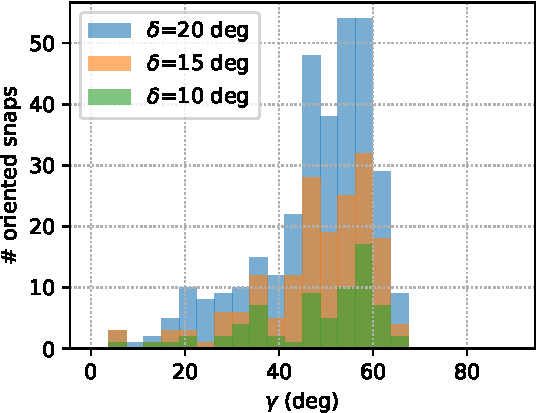
\includegraphics[width=0.8\columnwidth]{histo/multi_tol_vel_angle_bins_gauss90_25.pdf}
\caption{Distribution of the flight angle $\gamma$ of selected oriented snapshots with multiple tolerances $\delta$. $\gamma$ is defined as the angle between the galactic velocity vector in the the cluster reference frame and the line of sight direction.
%Overplotted a Kernel Desity Estimation for the distribution.
}
\label{fig:velocity_prediction}
\end{figure}
\begin{figure}
\centering
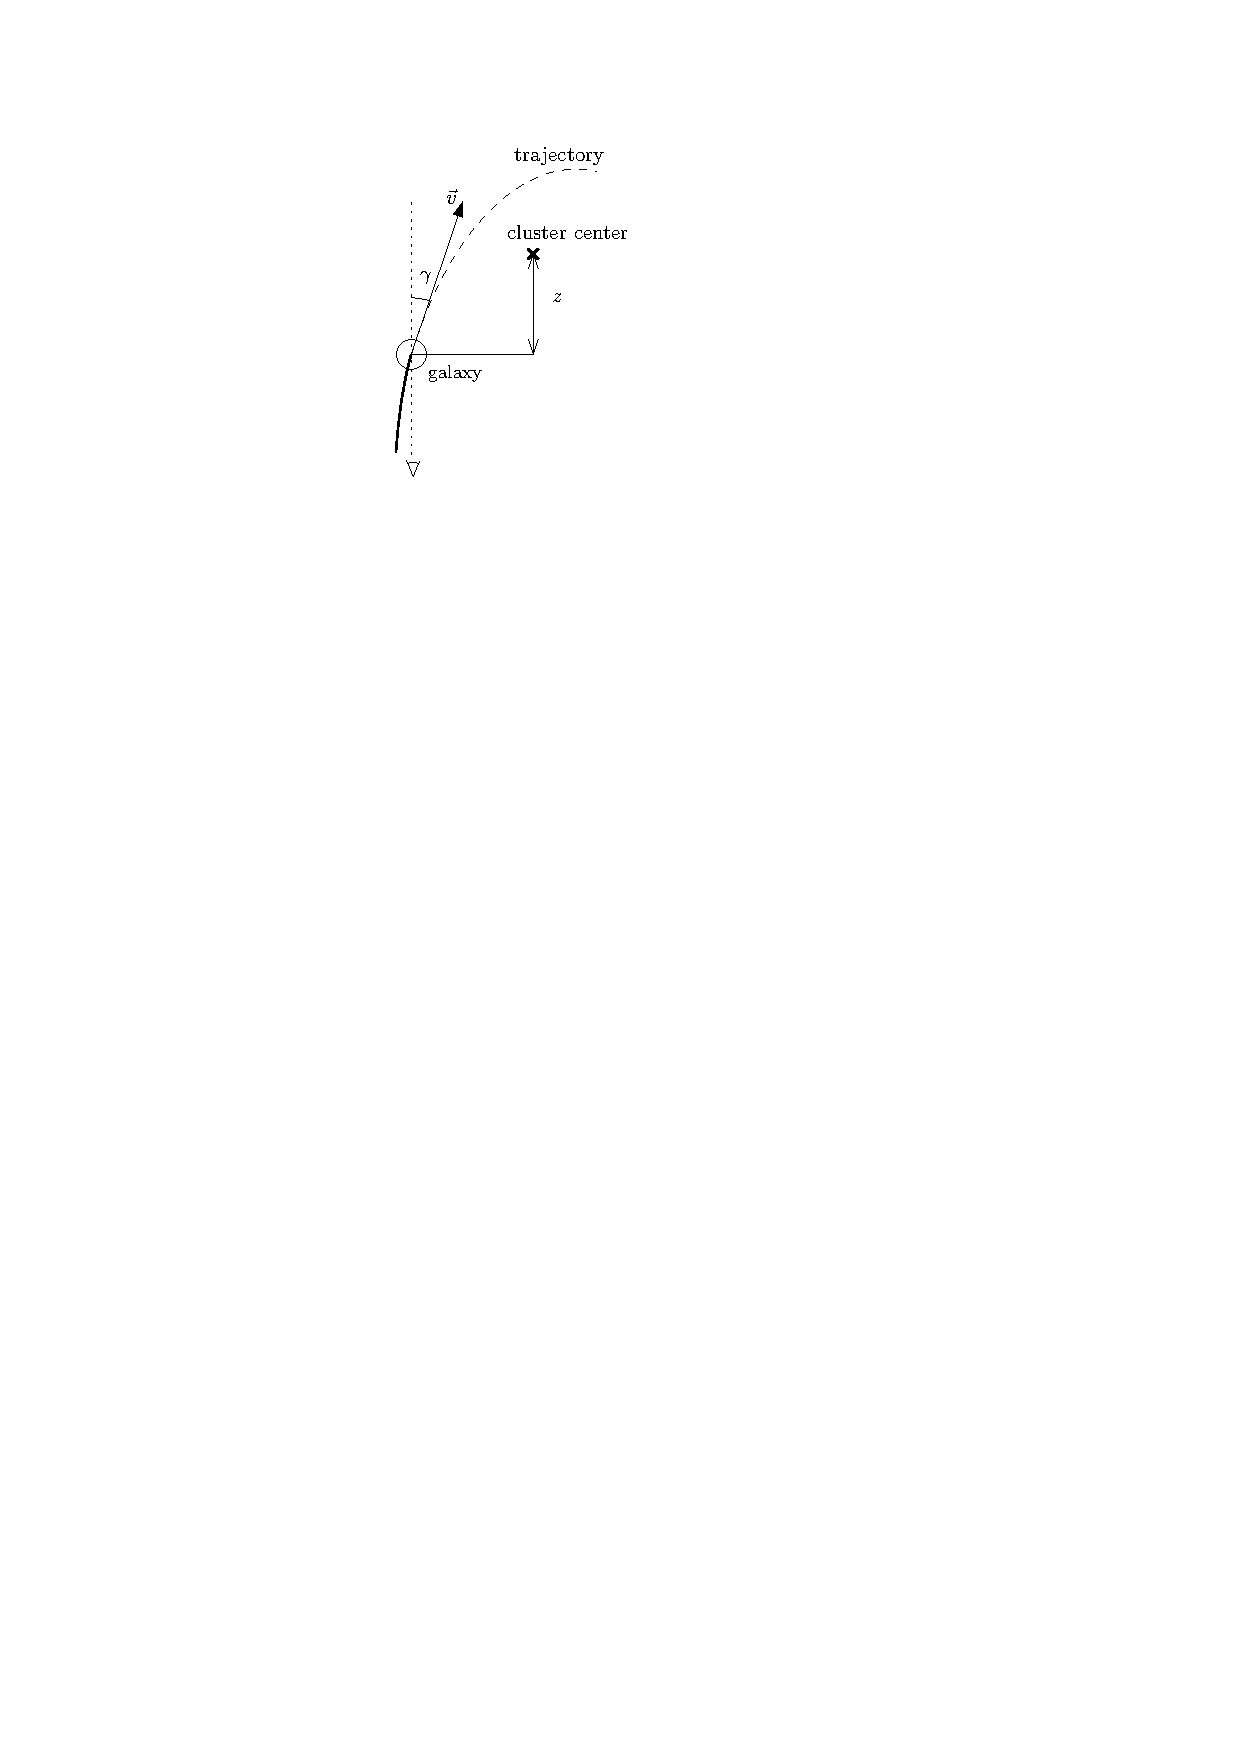
\includegraphics[width=0.5\columnwidth]{gamma.pdf}
\caption{Definitions of angle of flight $\gamma$ and radial distance $z$. $\vec v$ is the orbital velocity of the galaxy.
}
\label{fig:gamma}
\end{figure}

\section{Discussion} \label{sec:discussion}

\subsection{The asymmetric stellar tidal tails}

\subsubsection{Including asymmetry as a constraint}
As a way of quantifying the asymmetric stellar tides, we computed the non-parametric measure Asymmetry \citep[as defined by][]{Lotz2004} of our oriented snapshots. For each oriented snapshot we fed its surface brightness map to \verb|statmorph| \citep{Rodriguez-Gomez2019} isolating the region of the map within $27$~mag/arcsec$^2$.
As a reference, \citet{Su2021} find an Asymmetry of $0.23$ for NGC~1427A.
We tried to add the Asymmetry to the constraints described in Section \ref{sec:morphological_quest}. Given that almost all the oriented snapshots have an Asymmetry higher than $0.2$ \citep[in line with the average of $0.53\pm0.22$ for galaxies with intense star formation as reported by][]{Conselice2003}, we find that isolating snapshots at least as asymmetric as NGC~1427A do not affect the results.

By plotting Asymmetry on selected snapshots as a function of time from pericenter, as shown in Figure \ref{fig:histo2d_asym}, it can be seen that selected snapshots closer to the pericenter become more symmetric.
A possible reason of this can be hypothesised in the tidal pull close to the pericenter which squeezes the galaxy elongating it, hence removing asymmetric regions of the galaxies.
Indeed all simulations show an Asymmetry greater than the one of NGC~1427A. We note that this is in line with \citet{Rodriguez-Gomez2019} who find a systematically higher asymmetry for simulated galaxy of Illustris and Illustris~TNG \citep{Vogelsberger2014, Pillepich2018}, especially in the low mass range.
In fact, in a numerical simulation each star particle created represents stars of $\approx 1000$ \Msun{}: a simulated galaxy is always more "granular" than an observed real galaxy due to the limited resolution.

\begin{figure*}
\centering
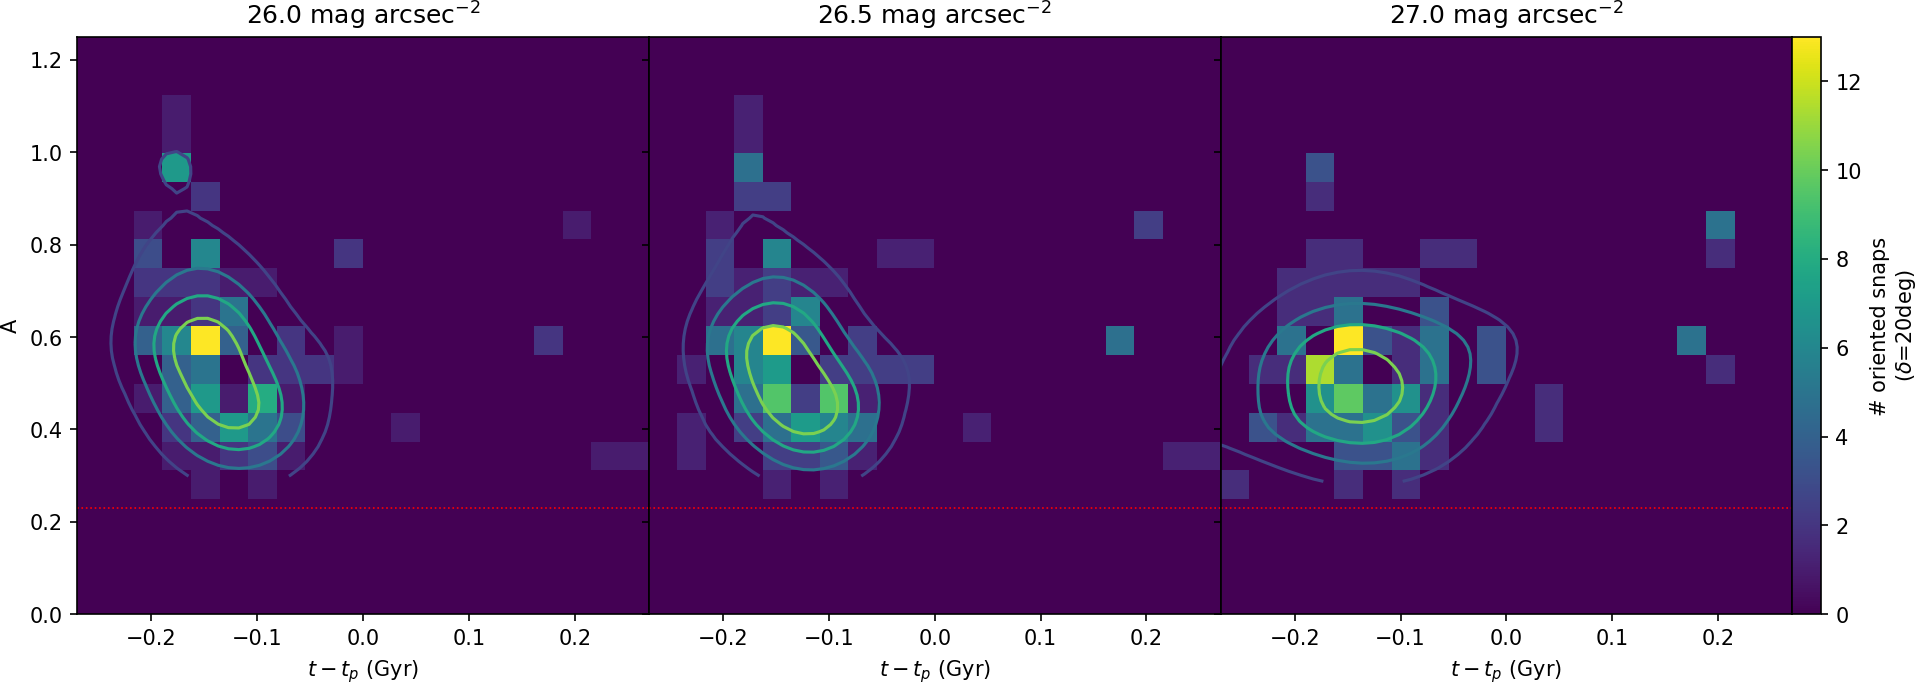
\includegraphics[width=\textwidth]{histo/hist2d_tp_A_bins20_kde-crop.png}
\caption{2D histogram of selected oriented snapshots with tolerance $\delta=20$~deg.
The distribution is plotted with time from first pericenter passage on the $x$ axis, whereas on the $y$ axis the \emph{Asymmetry} non-parametric measure as defined by \citet{Lotz2004}.
Each column corresponds to a different isophote used to compute the stellar tidal orientation.
We overplot a kernel density estimation of the distribution for the snapshots approaching pericenter. The dotted red line corresponds to the measured \emph{Asymmetry} for NGC~1427A.}
\label{fig:histo2d_asym}
\end{figure*}


% \subsubsection{Including isophotal twisting as a constraint}

\subsubsection{The origin of the asymmetric stellar tidal tails}
\begin{sidewaysfigure}
\centering
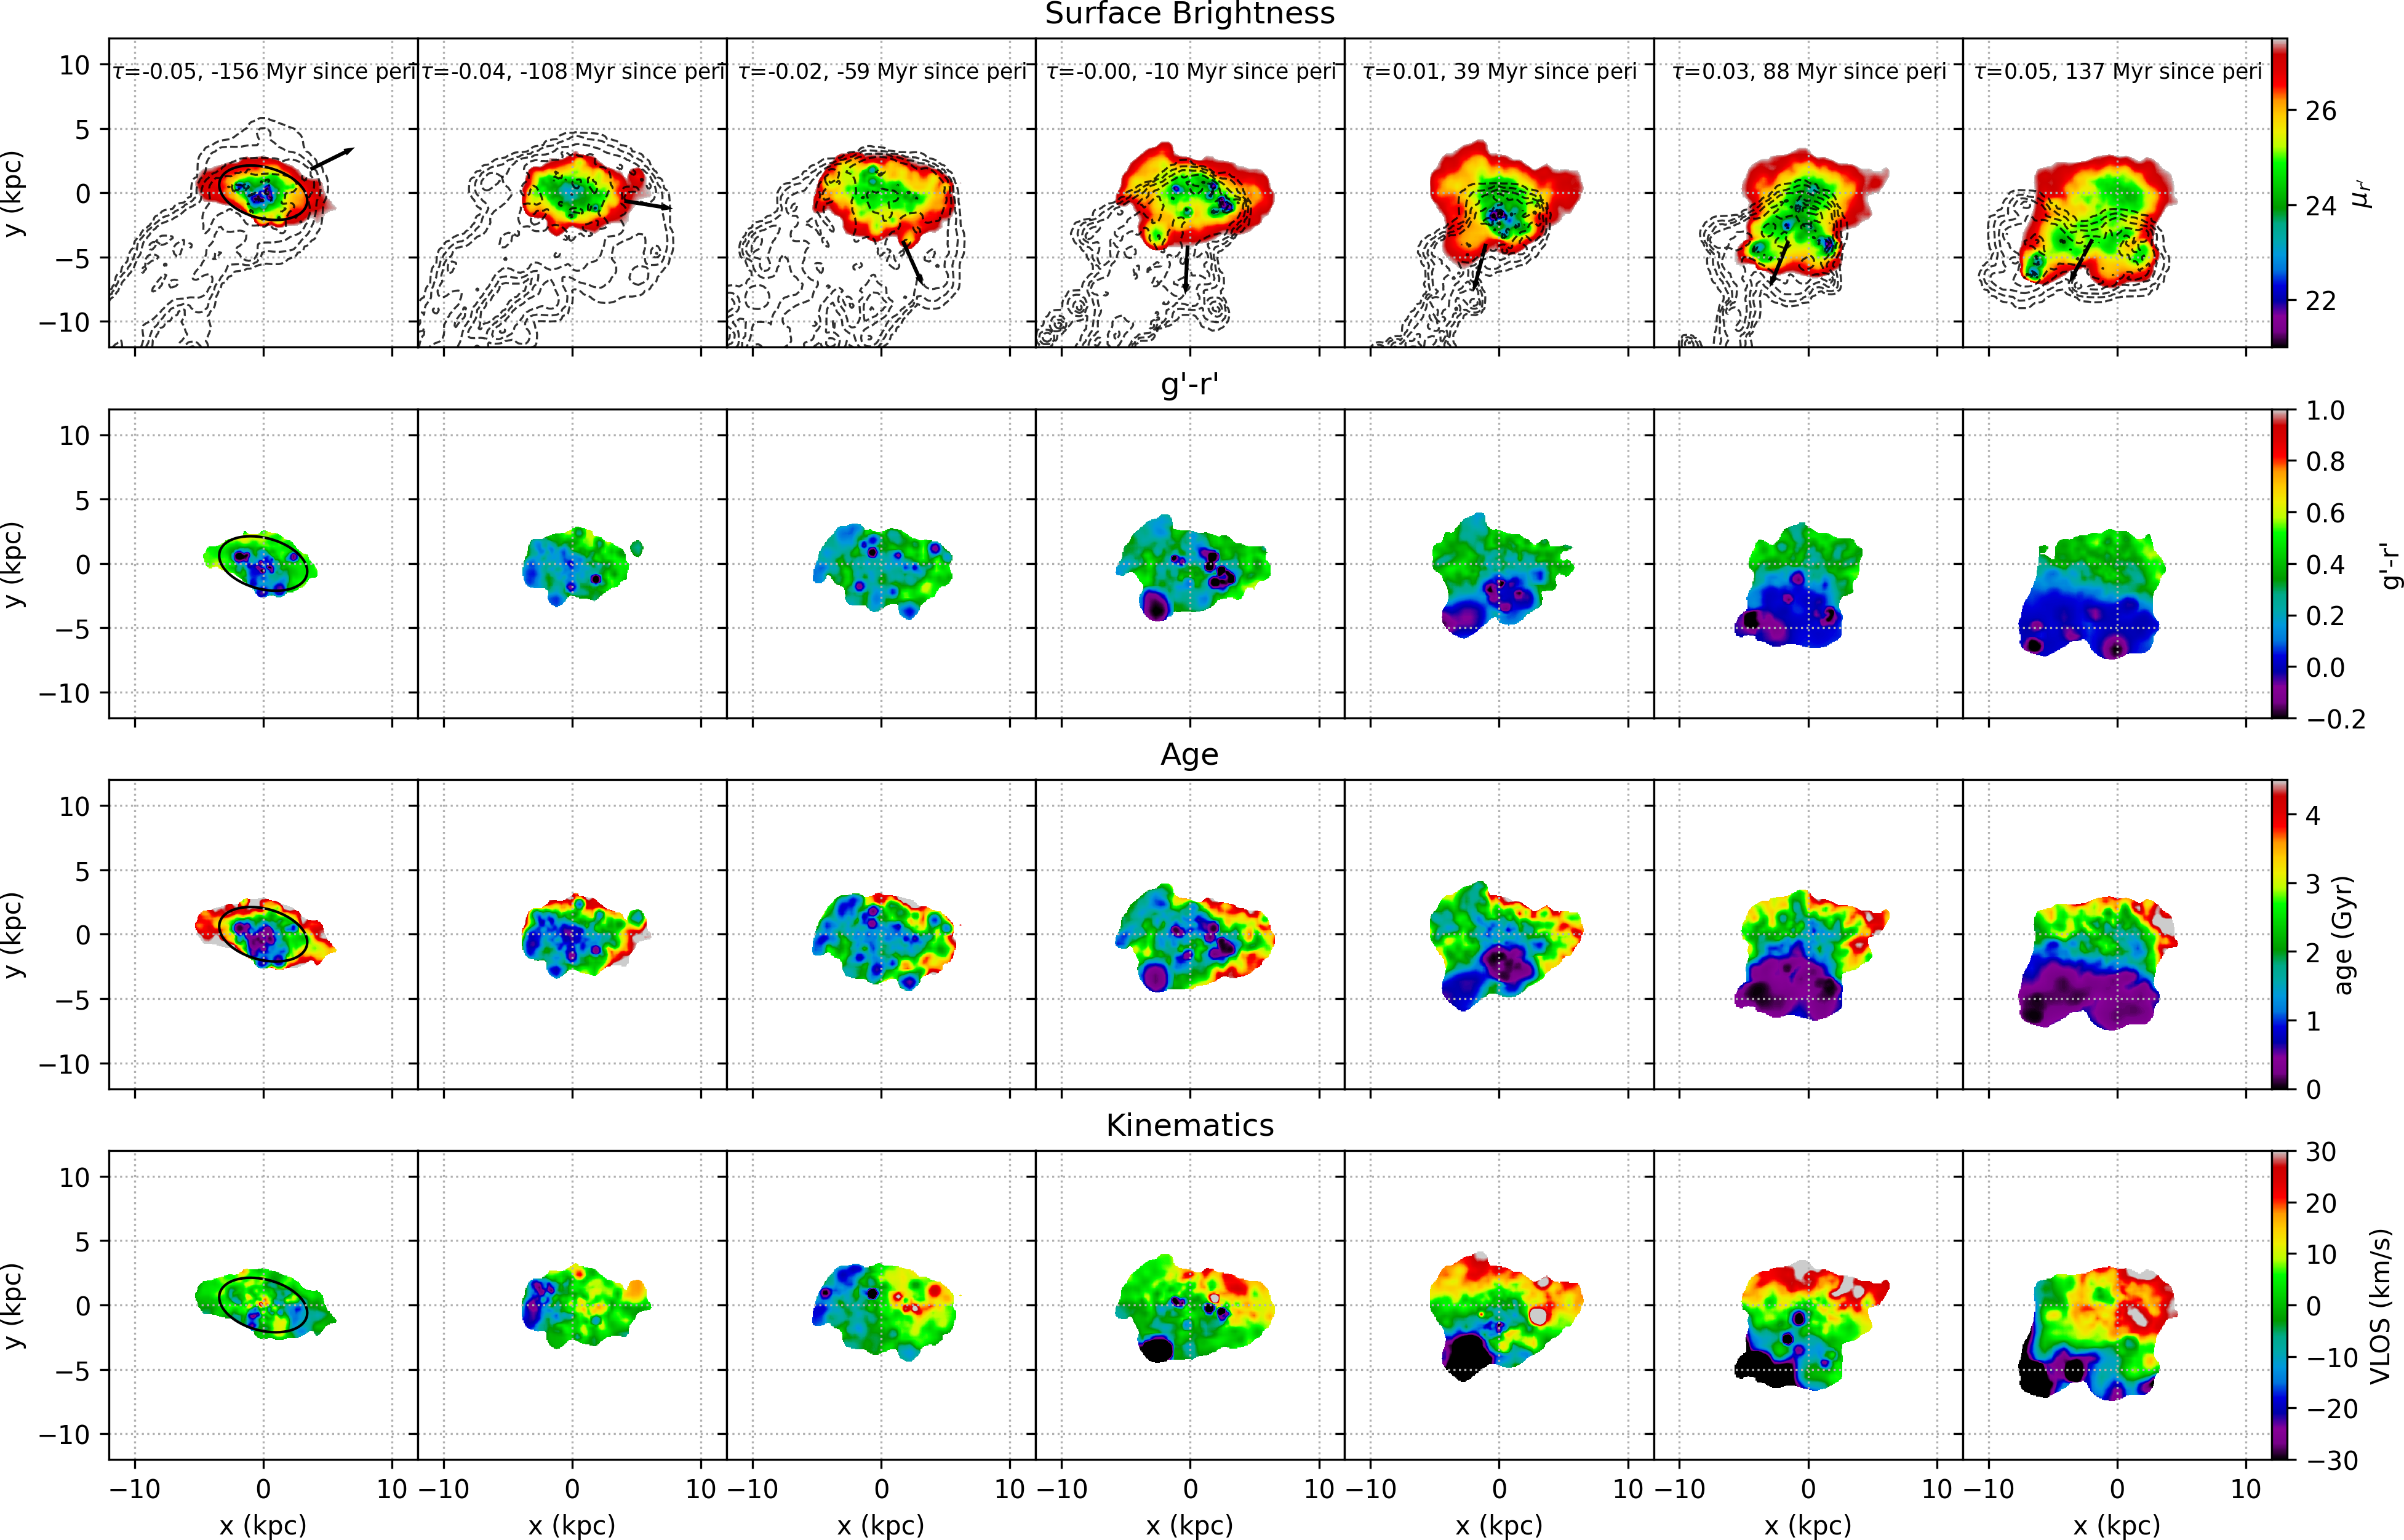
\includegraphics[width=0.95\textwidth]{panel68p100-crop.png}
\caption{Evolution in time of the simulation with ID 68 around first pericenter passage, projected in a way that the first column has $r_p = 137$~kpc, $v_p = 693$~km/s, the target values for NGC~1427A.
All the other snapshots are seen from the same point of view as the first one.
Black arrow indicates the direction to the cluster center whereas the green indicates the instantaneous velocity direction of the galaxy projected on the plane of the sky. In the first column, an ellipse fitted on the $26.5$ mag/arcsec$^2$ is shown to highlight the direction of the tidal elongation.
The first row represents the surface brightness of snapshots around the first pericenter. \Hi{} Contours are [$10^{17}, 10^{18}, 10^{19}, 10^{20}, 10^{21}$]~amu~cm$^{-2}$.
Second row the $g'$-$r'$ colour.
Third and fourth row the v-band SPH-average age and velocity of star particles along the line of sight.}
\label{fig:panel}
\end{sidewaysfigure}

An interesting effect of the pericenter passage is the formation of an asymmetric tidal tail, a stellar elongation more pronounced in just one direction, as that shown in the fourth column of Figure~\ref{fig:panel}.
This effect can be investigated by looking at different simulation snapshots evolving with time around a pericenter passage.
We focus our discussion to the case of the galaxy with ID 68 on an orbit with pericenter $100$~kpc.
In Figure~\ref{fig:panel}, the snapshot in the first column is the one who has passed the filters described in Section~\ref{sec:morphological_quest} and represents a snapshot which is in good agreement to the observation, given its stellar and gaseous tail directions and the projected clustercentric distance and recessional velocity.

We can then reconstruct a series of events leading to the generation of the leading edge stellar tail.
The tidal forces exerted by the Fornax Cluster become markedly asymmetric as a galaxy approaches pericenter on a radial orbit.
The steeply deepening gravitational potential well can raise a stronger leading stellar tidal tail while producing a weaker trailing tail during a fast swing-by of a galaxy close to the cluster center.
After pericenter, the leading tail twists due to the curvature of the galaxy's orbit, the rapidly changing direction of the gravitational force, and the internal rotation of the galaxy.
Effectively the pericenter passage injects energy into the galaxy resulting in a temporary increase of its angular momentum.

At the same time, the gaseous tail is always directed opposite to the instantaneous velocity.
The result is that the stellar and gaseous tails are very misaligned, almost orthogonal to each other.


\subsection{Possible origin of the Northern Clump in NGC 1427A} \label{NC1427A}
The galaxy NGC~1427A contains a so called Northern Clump (NC), which has been investigated in detail by some authors \citep{Cellone1997, Hilker1997}.
The NC is a clump of blue and very young stars with associated H$\alpha$ emission \citep{Sivanandam2014}.
Even on ground-based images, the NC appears to be composed of two sub-clusters, one to the north of the other.
This impression is strengthened by the HST image presented in Figure \ref{fig:NGC1427A}. The centers of the two sub-clusters are separated by 7'', corresponding to just under 700~parsec.
The NC lies on NGC~1427A's projected rotation axis and hence its line-of-sight velocity agrees very well with NGC~1427A's mean recession velocity \citep{Bureau1996,Chaname2000}. This does not hint at an external origin for this object.
The NC appears to be connected to the north-west rim of the galaxy's main body by a tenuous stream of stars, suggesting it to be displaced along this stream away from the galaxy's main body in a direction that is almost parallel to the major axis of the faint outer isophotes.
If, as in our interpretation of the data, these outer isophotes trace the two diametrically opposite stellar tides raised by the Fornax Cluster forces then this would argue for a purely internal origin of the NC.
It could be a star-formation region (of which there are many inside NGC~1427A) that is being pulled out by the Fornax Cluster tidal forces, leaving behind a stream of stars.
As shown in Figure \ref{fig:panel}, star formation flares up in our simulated dwarf galaxies around pericenter passage and leads to the appearance of scattered bright, blue clumps of active star formation.
These clumps orbit along with the general rotation of their host galaxy.
The spatial location and the time of appearance of these clumps are erratic and differ between galaxies and between orbits.
For instance, a star-forming clump is first visible to the top-right of the galaxy in the snapshots 108~Myr before pericenter passage (second column in Figure \ref{fig:panel};
it rotates clockwise, and disappears again after the 137~Myr past pericenter passage snapshot.
Likewise, other clumps with similar lifespans pop in and out of existence around pericenter passage.

Based on these simulations and the available observational data, we suggest that the NC is precisely such a star-forming clump. This interpretation is consistent with its very young age and blue colour, its presence around the time that NGC 1427A is expected to be near pericenter passage (this is required to explain all other characteristics of NGC 1427A), and its kinematics being in line with the galaxy's global velocity field.

%In simulations, as shown in Figure \ref{fig:panel}, around pericenter passage, star formation moves from the galactic center to the gas-rich tail because of ram pressure.
%Many clumps of young stars are therefore formed, suggesting a formation scenario for the Northern Object.
%After pericenter, the galaxy relaxes and stars are being formed again in the galaxy core.

\section{Conclusions}
We carried out a set of simulations of gas-rich late-type dwarf galaxies in a Fornax-like cluster environment.
We isolated snapshots with morphological properties similar to the peculiar galaxy NGC~1427A. The properties have been chosen to be representing the impact of the environment on the dwarf.
We found that the main effects generating peculiar morphology are indeed the combination of ram pressure and tidal interaction close to the cluster center and galaxy rotation.
We saw that the most likely scenario which recreates NGC 1427A tails morphology is assuming the galaxy to be on a very radial orbit with its tail almost aligned with the line of sight, pointing towards the observer.
This naturally leads to a gas kinematic configuration consistent with \Hi{} observations: in the westward part, gas attached to the stellar body of the galaxy is receding whereas the eastward part is stripped and dragged towards the observed by the intra-cluster medium (or ICM), therefore having a smaller recessional velocity, see Figures \ref{fig:sim_hi_kin} and \ref{fig:hi_kin}.

From the analysis of the morphology of the simulated snapshots motivated by environmental effects, we found an excess of snapshots revealing similar NGC~1427A structure around 150 Myr before pericenter passage.
It should be highlighted that this result comes from a suite of simulation which has not been tailored from the beginning to reproduce NGC~1427A.
Nonetheless, interestingly, falsifiable predictions on the location and orbital phase of the galaxy can be made.

We can sum up the main results in the following points:
\begin{itemize}
    \item Perpendicular gaseous and stellar tails are explainable given that they are subject to different environmental effects.
    \item Tails geometry is crucial to unravelling the direction of motion of the galaxy and its orbit.
    \item From our suite of simulation it is evident how around \textasciitilde 150~Myr before first pericenter passage, a morphological tail structure like the one of NGC~1427A emerges in galaxy falling into a Fornax-like cluster.
    \item In simulations, around pericenter, clumps of newly formed stars can form. This is coherent with a formation scenario of NGC~1427A's Northern Clump as a star formation region pulled out by tidal forces.
    \item Following our modelling it is possible to estimate the most likely position of a NGC~1427A-like galaxy to be around 200 kpc in front of the cluster center. Also, the most likely flight direction (represented by the angle $\gamma$ in the paper) is around 50~deg.
\end{itemize}

\section*{Data availability}
The data underlying this article and the algorithms used are available at this GitHub repository: \url{https://github.com/elehcim/ngc1427apaper}.

\section*{Acknowledgements}
Analysis of data and plots have been made possible thanks to open-source software:
\textsc{pynbody} \citep{Pontzen2013},
\textsc{numpy} \citep{numpy},
\textsc{scipy} \citep{scipy},
\textsc{pandas} \citep{pandas},
\textsc{matplotlib} \citep{Hunter2004},
\textsc{astropy} \citep{TheAstropyCollaboration2018},
\textsc{statmorph} \citep{Rodriguez-Gomez2019}.
